
\chpt{Analysis} \label{ChapterAnalysis}


%% Flux definition 
In this chapter, the details of the antiproton analysis will be given, including all the steps of deriving the time-averaged and time-dependent antiproton to proton flux ratio. To determine the flux ratio, the definition of flux should be given first. In general, the flux as a function of true rigidity is calculated by: 

\begin{equation}
\label{FluxCalculationEquation}
\Phi(|R|_{\rm{true}}) = \frac{N(|R|_{\rm{true}})}{\Delta R \cdot T(|R|_{\rm{true}}) \cdot A(|R|_{\rm{true}}) \cdot \epsilon(|R|_{\rm{true}}) }
\end{equation}

where $N(|R|_{\rm{true}})$ is the number of events in this rigidity bin, $\Delta R$ is the rigidity bins width, $T(|R|_{\rm{true}})$ is the measuring time, $\epsilon(|R|_{\rm{true}})$ is the trigger efficiency and $A(|R|_{\rm{true}})$ is the effective acceptance. The quantities in equation \ref{FluxCalculationEquation} are as a function of true rigidity, while the number of events, derived from the template fit (a method to extract signal and background events from the total event distribution, see Section \ref{TempalteFitSection}), is expressed as a function of reconstructed rigidity. To get the event number in true rigidity, a procedure called "unfolding" is performed. This will be discussed further in section \ref{unfoldingsection}.  \par


%% Time Averaged: Antiproton to Proton flux ratio
In this thesis, the objective is the antiproton to proton flux ratio. Therefore, the dedicated formula should be determined based on the equation \ref{FluxCalculationEquation}. Given the antiproton and proton flux definitions:

\begin{equation} 
\begin{aligned}  
\Phi_{\bar{p}}(|R|_{\rm{true}}) =  \frac{N_{\bar{p}}(|R|_{\rm{true}})}{\Delta R_{\bar{p}} \cdot T_{\bar{p}}(|R|_{\rm{true}}) \cdot A_{\bar{p}}(|R|_{\rm{true}}) \cdot \epsilon_{\bar{p}}(|R|_{\rm{true}}) }\\
\Phi_{p}(|R|_{\rm{true}}) =  \frac{N_{p}(|R|_{\rm{true}})}{\Delta R_{p} \cdot T_{p}(|R|_{\rm{true}}) \cdot A_{p}(|R|_{\rm{true}}) \cdot \epsilon_{p}(|R|_{\rm{true}}) }
\end{aligned}
\end{equation}

the antiproton to proton flux ratio is defined as the antiproton flux divided by the proton flux. In this process, some terms can be strictly canceled out, like in the AMS-02 positron to electron flux ratio analysis \cite{ZimmermannPhDThesis}. Therefore, the overall calculation can be simplified:

\begin{equation} 
\begin{aligned}  
\frac{\Phi_{\bar{p}}(|R|_{\rm{true}})}{\Phi_{p}(|R|_{\rm{true}})} &= \frac{N_{\bar{p}}(|R|_{\rm{true}}) \cdot \Delta R_{p} \cdot T_{p}(|R|_{\rm{true}}) \cdot A_{p}(|R|_{\rm{true}}) \cdot \epsilon_{p}(|R|_{\rm{true}}) }{ N_{p}(|R|_{\rm{true}}) \cdot \Delta R_{\bar{p}} \cdot T_{\bar{p}}(|R|_{\rm{true}}) \cdot A_{\bar{p}}(|R|_{\rm{true}}) \cdot \epsilon_{\bar{p}}(|R|_{\rm{true}}) } \\ 
&= \frac{N_{\bar{p}}(|R|_{\rm{true}}) \cdot A_{p}(|R|_{\rm{true}})}{N_{p}(|R|_{\rm{true}}) \cdot A_{\bar{p}}(|R|_{\rm{true}})} \\ 
&= \frac{N_{\bar{p}}(|R|_{\rm{true}}) \cdot A^\mathrm{MC}_{p}(|R|_{\rm{true}}) \cdot (1+\delta_{p}(|R|_{\rm{true}}))}{N_{p}(|R|_{\rm{true}}) \cdot A^\mathrm{MC}_{\bar{p}}(|R|_{\rm{true}}) \cdot (1+\delta_{\bar{p}}(|R|_{\rm{true}}))} \\ 
& = \frac{N_{\bar{p}}(|R|_{\rm{true}}) \cdot A^\mathrm{MC}_{p}(|R|_{\rm{true}})}{N_{p}(|R|_{\rm{true}}) \cdot A^\mathrm{MC}_{\bar{p}}(|R|_{\rm{true}})}
\end{aligned}
\label{PbarOverProtonRatioEquation}
\end{equation}

where $A^{\mathrm{MC}}_{p}(|R|_{\rm{true}})$ and $A^{\mathrm{MC}}_{\bar{p}}(|R|_{\rm{true}})$ are the effective acceptances of proton and antiproton taken from the MC, $\delta_{p}(|R|_{\rm{true}})$ and $\delta_{\bar{p}}(|R|_{\rm{true}})$ are the data/MC corrections of the proton and antiproton effective acceptances, more details about these will be given in section \ref{EffectiveAcceptanceSection}. As shown in equation \ref{PbarOverProtonRatioEquation} the terms that cancel out in the antiproton to proton flux ratio are the rigidity bin width $\Delta R$, the measuring time $T(|R|_{\rm{true}})$, the trigger efficiency $\epsilon(|R|_{\rm{true}})$ and the data/MC corrections of the effective acceptance $(1+\delta(|R|_{\rm{true}}))$. The details of these terms will be shown in detail in the following sections. These cancellations simplify the calculation of the antiproton to proton flux ratio.  \par
% Although the measuring time and the trigger efficiency cancel out in the ratio calculation, they are still used in the unfolding process. 


%% Time Dependent: Antiproton to Proton flux ratio
For the time-dependent antiproton to proton flux ratio calculation, the formula in time bin $i$ is given in Equation \ref{TimeDependentPbarOverProtonRatioEquation}, which is similar to the time-averaged one. The difference is that the number of events is obtained from the individual template fits in every six Bartels Rotation time bin. \par

\begin{equation} 
\begin{aligned}  
\frac{\Phi_{\bar{p},i}(|R|_{\rm{true}})}{\Phi_{p,i}(|R|_{\rm{true}})} &= \frac{N_{\bar{p},i}(|R|_{\rm{true}}) \cdot \Delta R_{p,i} \cdot T_{p,i}(|R|_{\rm{true}}) \cdot A_{p,i}(|R|_{\rm{true}}) \cdot \epsilon_{p,i}(|R|_{\rm{true}}) }{ N_{p,i}(|R|_{\rm{true}}) \cdot \Delta R_{\bar{p},i} \cdot T_{\bar{p},i}(|R|_{\rm{true}}) \cdot A_{\bar{p},i}(|R|_{\rm{true}}) \cdot \epsilon_{\bar{p},i}(|R|_{\rm{true}}) } \\ 
& = \frac{N_{\bar{p},i}(|R|_{\rm{true}}) \cdot A^\mathrm{MC}_{p,i}(|R|_{\rm{true}})}{N_{p,i}(|R|_{\rm{true}}) \cdot A^\mathrm{MC}_{\bar{p,i}}(|R|_{\rm{true}})}
\end{aligned}
\label{TimeDependentPbarOverProtonRatioEquation}
\end{equation}


%% Content of Analysis Chapter
In section \ref{DataSelectionSection}, the cuts and selections are discussed. Section \ref{chargeconfusion} shows the construction of the charge confusion estimator. Section \ref{TRDEstimatorSection} describes how the TRD likelihood estimator is constructed. In section \ref{TempalteFitSection}, the template fit procedures to get the antiproton signals in different rigidity ranges are shown. Section \ref{EffectiveAcceptanceSection} gives the details about how to calculate the effective acceptances of antiproton and proton. In section \ref{MeasuringTimeSection}, the measuring time used in this analysis is determined. Although the measuring time is canceled in the antiproton to proton flux ratio calculation, it has to be calculated because the rigidity cutoff is not simulated in the MC simulation which is used for unfolding, also the measuring time in the time-dependent analysis is important to understand the event numbers change. Section \ref{unfoldingsection} shows the unfolding procedure. In section \ref{SecAntiprotonToProtonRatio}, the antiproton to proton flux ratio is given with statistical uncertainty only. In section \ref{SystematicUncertaintiesSection}, the different systematic uncertainties in different rigidity ranges are discussed.  \par

%In section \ref{TriggerEfficiencySection}, the trigger efficiency used in this analysis is calculated.
%In section \ref{SecAntiprotonToProtonRatio}, the formula for the calculation of antiproton to proton flux ratio is derived. 


\section{Data Selection} \label{DataSelectionSection}

% SubSection 1: General Description 
\subsection{AMS-02 Data and Monte Carlo Simulation}

%% ISS data
This section provides information on the data used in this analysis and presents the complete list of cuts and selections. In this analysis, the AMS-02 experiment data has been collected from May 20th 2011 to May 3rd 2021. Collected raw data need some calibration and alignment work and then can be reconstructed via the AMS-02 official software (named gbatch), resulting in the analysis data stored in ROOT files. The ROOT data analysis format is developed at CERN and it is dedicated for High energy particle physics analysis \cite{CERNROOTPaper}. Furthermore, a software package developed in Aachen called ACSoft is used to further process and store the data in a higher-level structure called ACQT \cite{BastianPhDPaper}. The analysis in this thesis is based on the so-called pass7 version of data (reconstructed via gbatch in version B1130). \par

%% Rigidity Bins 
The rigidity binning used in this analysis is the same as the one used in the previous AMS-02 proton analysis \cite{AMS02ProtonPaper}, which is determined by the rigidity resolution. At the rigidity regions higher than 80.5 GV, the rigidity bins are merged in every two bins to increase antiproton statistics.  \par

%% ISS data for Time Dependent Analysis  (Bartels Rotations)
%The sun is not a solid body but is made of gas plasma. Due to the solar rotations, different latitudes would show different rotation periods. From the view of the Earth, the solar rotations can be quantified with the Bartels Rotation Numbers. One Bartels Rotation Number is equal to exactly 27 days, close to the synodic rotation period \cite{BartelsRotationBook}. The counting of the Bartels Rotations started on February 8th 1832, a day that was arbitrarily assigned by Julius Bartels.   \par

For the time-dependent analysis, the collected ISS data is divided into six Bartels Rotations time bins. A Bartels Rotation is exactly 27 days, close to the synodic rotation period of the Sun. Because of the rigidity cutoff, the statistics in the low rigidity range in each time interval is limited. Therefore, the rigidity bins are also merged in every two original time-averaged rigidity bins in time-dependent antiproton analysis. The data collection used in this thesis started in May 2011, which corresponds to the Bartels Rotation 2426, and ended in May 2021, at the Bartels Rotation 2561. In total, the data can be divided into 23 intervals of six Bartels Rotations each though the last time bin has less data than the full six Bartels Rotations.  \par

%% TTCS 
Due to the upgrade of the cooling system of the AMS silicon tracker that took place from Nov 2019 to Jan 2020, the operation mode frequently changed during some periods as the cooling system pump had to be switched off. The data collected during these time periods is excluded and not used in this analysis. \par

%% MC data 
To validate the sub-detector's performance and study the detector's operation, an extensive set of MC simulations has been produced by the AMS-02 collaboration with the help of the Geant4 framework \cite{GEANT4Paper1, GEANT4Paper2}. The Geant4 is a software toolkit that simulates the passage of particles through matter. The interactions of the cosmic ray particles with all the AMS-02 sub-detectors and their support structure can be studied with this toolkit. By comparing the data distributions for different variables between MC and ISS data, the sub-detector's response to different cosmic rays can be systematically studied. \par   


%% comment: all the MC datasets used in this analysis. 
\begin{comment}  	

1. For CC training and CCProton Template:
B1042_pr.pl1.flux.l1a9.2016000_7.6_all
B1042_pr.pl1.flux.l1o9.2016000_7.6_all

2. For acceptance:
Proton:
B1042_pr.pl1.1800_7.6_all
Antiproton:
B1042_antipr.pl1.1800_7.6_all
B1220_antipr.pl1ph.021000.qgsp_bic_ams.plus10_7.8_all
B1220_antipr.pl1ph.021000.qgsp_bic_ams_7.8_all		
B1220_antipr.pl1ph.021000.qgsp_bic_ams.minus10_7.8_all	

3. Electron:
B1091_el.pl1.0_25_2000_7.6_all_merged	
B1091_el.pl1.0_25200_7.6_all		
B1091_el.pl1.2002000_7.6_all	

4. Data:
B1130_pass7	

others:	
B1220_pr.pl1ph.021000_7.8_all	
B1220_pr.pl1phpsa.0550.4_00_7.8_all	
B1220_pr.pl1phpsa.l19.5016000.4_00_7.8_merged 
B1220_pr.pl1phpsa.l1o9.flux.2016000.4_00_7.8_all
B1200_el.pl1.120_7.8_all	

\end{comment}		
	
%% MC data Usage: 1. CC estimator.  2. systematic error of acceptance 3. acceptance
%In this thesis, the MC datasets used are for protons, antiprotons, and electrons. 
In this thesis, the used MC datasets are:
\begin{itemize}
\item B1042 Protons MC with generated momentum from 20 to 16000 GeV
\item B1042 Protons MC with generated momentum from 1 to 800 GeV
\item B1042 Antiprotons MC with generated momentum from 1 to 800 GeV
\item B1220 Antiprotons MC with generated momentum from 0.2 to 1000 GeV 
\item B1091 Electrons MC with generated momentum from 0.25 to 200 GeV
\item B1091 Electrons MC with generated momentum from 200 to 2000 GeV
\end{itemize}

\begin{figure}[H]
\centering
\includegraphics[width=1.0\textwidth]{Figures/chapter4/DataSelection/{B1042_antipr.pl1.1800_7.6_all_mc_iss_ratio}.pdf}
\caption[The antiproton statistics comparison between MC and ISS data.]{The statistics comparison between antiproton numbers from MC simulation and antiproton events from ISS data. The jumps in the ISS data are due to the different selections in different rigidity ranges. The statistics of antiproton MC is at least ten times larger than the antiproton events from ISS data.}
\label{MCISSStatisticsCompare}
\end{figure}

%657: discuss the jumps in the spectral shapes

In figure \ref{MCISSStatisticsCompare}, the statistics of antiproton MC simulation and the antiproton events from the ISS data (which will be given in the following sections) are shown. The antiproton MC statistics is at least ten times larger than the antiproton events determined from the ISS data.        \par

Different MC datasets are generated in different momentum ranges for various purposes. For example, one of the main purposes of using MC proton data in this analysis is to study the proton charge confusion events, which are proton events but measured with the wrong rigidity sign. The reasons are finite tracker rigidity resolution and the interactions with the sub-detectors \cite{ChargeConfusionReasonsAndTrackerResolutionPaper}. By selecting the negative rigidity data samples from the proton MC dataset, the proton charge confusion events can be studied. This issue will be discussed in more detail in Section \ref{chargeconfusion}. The MC datasets are also used for other purposes like calculating effective acceptance and determining the systematic uncertainties due to acceptance, these will be shown in detail later in this chapter.    \par  

%% MC data reweighting
For the simulated MC events, the generated momentum spectrum does not perfectly match the real cosmic spectrum. This could introduce bias in some variable distributions in MC. In order to correct this, the weight of each event in a MC dataset has to be reassigned by making the flux computed from this MC dataset equal to a reference flux. For example, the AMS-02 published proton flux result \cite{AMS02ProtonPaper} is used as the reference flux for proton MC datasets. The acquired re-weighting factor will be used in filling variable histograms for further study.  \par  

%\begin{equation}
%w=\frac{\phi}{MC}
%\end{equation}

%Fabian:
% To correct this, a weight is determined for each event such that a flux computed from the MC events is equal to a reference flux. In this analysis, a model for the electron flux is used as a reference (Appendix A.2) and the protons are assumed to follow a power law with a spectral index of γ = −2.7 and solar modulation calculated according to the force field approximation (equation 2.4) with a potential of φ = 500 MV.
%Manbing:
% To get a realistic distribution of MC data, reweighting of each event is applied. This is done using the flux spectrum measured by AMS [14] as a scaler. Figure 4.5 presents the lithium MC event weights as a function of the true rigidity.
% With the weight factors, the MC rigidity spectrum has the same shape as the data sample.
%Mine_old:
%In order to correct this, the weights of MC events are reassigned by making the spectrum of MC simulation is same as the reference one. 


%% Introducing data selection
Up to May 2021, the AMS-02 experiment has collected more than 174 billion cosmic ray events. To select antiproton events from them, cuts and event selections are applied. There are two levels of selection; the first one is the so-called “Preselection” and the second one is the more refined “Selection”. In the next few subsections, the definition of all selections and their pass ratios will be given. The pass ratio is the event number passed in this cut to the total event number before applying the selector (a group of cuts at this level of selection) to which this cut belongs. \par 
%676: the "pass ratio" is not well defined. What exactly is the denominator? Events before all cuts? After the previous cut? ...?

%  SubSection 2. : Preselection
\subsection{Preselection Cuts}
The first level of cuts and selections is the preselection. The purpose is to discard data taken during bad sub-detectors operation conditions or have bad quality. These selections are general and applied before any cosmic ray component AMS-02 analyses. The preselection consists of two parts: data taking quality cuts and analysis data quality cuts. Each part is a selector. \par 

%% 2.1 Preselection: data taking quality cuts
Data taking quality cuts require all the sub-detectors running in nominal conditions, and the data taking conditions are normal. The first one excludes the period that any sub-detector operates under special conditions or undergoes testing. For example, the TRD gas refill procedure takes place once per month. In this period, the data taken is not included in this analysis. The second one requires that the data taking period is normal. For instance, if the ISS is in the SAA area, the data taken in this period is not included in this analysis. In summary, Table \ref{data taking quality cuts} shows the pass ratios of all the data taking quality cuts. \par
%The pass ratio is defined as the ratio of event numbers passed in this cut to the total event numbers before applying the cuts in the list.


\begin{table}[tp]
\renewcommand\arraystretch{1.3}
\caption{List of data taking quality cuts and their pass ratios}
\label{data taking quality cuts}
\begin{tabular}{l p{7.5cm}  c} 
\hline
Cuts & Description & Pass Ratio \\
\hline

\textbf{Bad Runs}                                &  Remove the events collected when the sub-detector is in unstable condition, for example the TRD gas refill period or when the DAQ was unavailable.                & 99.73 \% \\
%RTI data Available                & RTI info available for second                                      & 100    \% \\
%Most Events Triggered         & Most events in second triggered                                 & 100    \% \\
\textbf{Second Within Run}                 & Remove the events collected without a run ID.            & 99.92  \% \\
\textbf{Bad Reconstruction Period}     & Remove the events collected in low reconstruction efficiency. The number of reconstructed events over the trigger rate should be nominal, otherwise the reconstruction efficiency is very low.                            & 95.15  \%  \\
\textbf{Bad Facing Angle}                    & Remove the events collected when the zenith angle of the ISS is larger than $40^{\circ}$.                              & 99.78  \% \\
\textbf{No Missed Events}                   & Remove the seconds if there are more than 10\% events missing in this second. This situation could result from transferring problems in the DAQ boards or buffer overflows issues.                                                         &    99.91 \% \\
\textbf{Bad Live Time}                         & Remove the seconds when the live time fraction (see Section \ref{MeasuringTimeSection}) < 0.5.        & 95.67  \% \\
\textbf{Too Many Events In Second}   & Remove the seconds if it contains more than 1800 reconstructed events. The rejected events are mostly taken from the SAA area or near the pole regions.                     & 97.86  \% \\
\textbf{Good Alignment}                      & Remove the seconds when the external tracker planes are not in good alignment. The shifts of the external tracker planes to be corrected are estimated by different AMS-02 groups and they should be consistent.                     & 99.86  \% \\
\textbf{High TRD Occupancy Period}  & Remove the seconds when the TRD occupancy is very high, namely the mean number of recorded TRD hits per second is larger than 1000.                             & 97.80   \%  \\
\textbf{No Hardware Errors}                & Remove the seconds when the hardware errors are detected, for example the bit-flips in the electronic boards.      & 99.91   \% \\
%TrdCalibrationAvailable        & Full TRD Calibration available                                   & 100      \% \\
\hline
\end{tabular}
\end{table}


\begin{comment}  	
Bad Runs 
2. Nominal data taking period
The AMS-02 collaboration keeps track of time intervals in which the detector was in an unstable condition, such as the first weeks of commissioning, all periods where the TRD gas system is refilled, when the DAQ was unavailable, etc. These so-called “bad runs” are excluded when analyzing the ISS data.

Bad Reconstruction Period 
1. Nominal reconstruction period
The ratio of reconstructed particles over the trigger rate in each second should be nominal.
Figure A.1 shows a plot of the trigger rate as function of the ratio: reconstructed particles over
the trigger rate. The red dashed line y = 1600 · x separates the nominal reconstruction period 0.07
from the non-nominal reconstruction period, where the reconstruction efficiency is low. All entries left of the line are rejected for further analysis.

Bad Facing Angle
4. Nominal ISS zenith angle
The zenith angle of the ISS must be less than 40°. Periods when the ISS was rotated must be excluded for analysis.

No Missed Events 
5. No missed events
If there are more than 10 \% of the events missing in a second, exclude the second for analysis. 
There are rare reasons that can lead to missing events, for instance transfer problems in the DAQ boards, or buffer overflows on the data reduction boards.

Bad Live Time
8. Nominal live-time
If the detector was busy for more than 50 \% in a second, reject the time period.

Too Many Events In Second
7. Too many events in second
If the amount of reconstructed events exceeds 1800 in a second, reject the time period. Events in these conditions are mostly taken near the SAA [Kurnosova1962] or in the pole regions, where the detector is filled with low energy particles. These periods should be rejected.

Good Alignment  
6. Good tracker alignment
The tracker alignment of the external tracker planes (Layer 1 and Layer 9) is performed independently by the Perugia and CIEMAT groups. Both alignment procedures should yield a similar set of alignment parameters for a given time period. Two important parameters are the shifts of the whole tracker plane with respect to the inner tracker: ∆X and ∆Y. If the ∆X or ∆Y in Layer 1 between the Perugia / CIEMAT method differs by more than 70 μm the time period is excluded. Likewise if the ∆X or ∆Y in Layer 9 differs by more than 100 μm the time period is excluded as well.

High TRD Occupancy Period
10. Nominal occupancy in TRD
Usually, the mean number of hits recorded in the TRD in each second is ≈ 60. If the mean number of hits per second exceeds 1000, the second will be rejected. This happens frequently at the edges of the SAA or in the pole regions.

No Hardware Errors  
9. Nominal DAQ condition
If hardware errors were detected in the second, reject it. Hardware errors might be bit-flips in the electronic boards, or duplicated events that got recorded, due to problems in the DAQ.

~~~~~~~~~~~~~~~~~~~~~~~~~~~~~~~~~~~~~~~~~~~~~~~~~~~~~~~~~~~~~~~~~~~~~~
My but not in Nico's:
Second Within Run   

Nico's but not in mine:
%3. Nominal trigger performance
%The amount of recorded events in each second of ISS data must be compatible with the expectation from the trigger rate: ftrigger/Nevents > 0.98
\end{comment}  	




%% 2.2 Preselection: analysis data quality cuts
The data taking quality cuts ensure that the events selected were collected during normal operation time periods, but for analysis, further quality selections are needed to ensure the analysis based on these data is meaningful. The analysis data quality cuts are used to discard the bad quality collected data. In Table \ref{analysis data quality cuts}, the complete list of the analysis data quality cuts and their correspondent pass ratios are shown. The definitions of analysis data quality cuts are the following:  

\begin{table}[ht]
\renewcommand\arraystretch{1.3}
\centering
\caption{List of analysis data quality cuts and their pass ratios}
\label{analysis data quality cuts}
\begin{tabular}{lc}
\hline
Cuts  & Pass Ratio \\
\hline
% only high: TrackerTrackInEcalAcceptance
% only low:  CutPhysicsTriggerChargedParticles, CutTofNumberOfLayers, CutRigidityAboveGeomagneticCutoff.  
%Has at least one analysis particle                          & 99.95 \% \\
%Trigger information available                                  & 99 \% \\
%%%%Has TOF Beta Measurement                        & 68.02  \%  \\        (old, merged then)
%%%%Particle is Downgoing                                   & 88.03 \%   \\        (old, merged then)
\textbf{Particle is Downgoing}                                               & 59.84 \% \\
%Has Tracker Track                                                    & XX \%\\
%Has Tracker Track Fit                                               & 69.52 \% \\
%HasTrackerTrackCoordinates                               & 100 \% \\
\textbf{Has Hits in Central Inner Tracker}                              & 70.16 \% \\
%Has charge measurement in inner Tracker             & 100 \% \\
%Has TOF charge measurement                              & 100 \%\\
\textbf{Has Single Tracker Track}                                        & 61.01 \% \\
\textbf{Tracker Track Fit $\chi^2$ in X}                                       & 97.33 \% \\
\textbf{Tracker Track Fit $\chi^2$ in Y}                                     & 90.64 \% \\
\textbf{Has Hits in all four TOF Layers}                                   & 89.44 \% \\
%Rigidity Above Geomagnetic Cutoff                    & XX \% \\
\hline
\end{tabular}
\end{table}           

\begin{itemize}
%\item The \textbf{Has TOF Beta Measurement} requires that the TOF beta measurement is available. The TOF beta is used to separate antiproton signals and backgrounds in low rigidity ranges.
%\item The \textbf{Particle is Downgoing} is the cut on particle going direction. By requiring TOF beta measurement is positive, the particle going from upper TOF to lower TOF is selected. 
\item The \textbf{Particle is Downgoing} is the cut on the particle’s moving direction. By requiring that the TOF has $\beta$ measurement and the TOF $\beta$ to be positive, particles moving from the upper TOF to the lower TOF are selected. In this way, the particle's going direction from the top of the instrument to the bottom is achieved. 
%\item The \textbf{Has Tracker Track Fit} is the cut on events that have fitted tracker tracks. 
\item The \textbf{Has Hits in Central Inner Tracker} requires hits in the tracker layers 3 or 4, 5 or 6,  7 or 8. To have an accurate rigidity measurement, the tracker hits inside the magnet are necessary. Therefore the central inner tracker should have enough hits for the rigidity measurement.    
\item The \textbf{Has Single Tracker Track} requires that for each event, only one reconstructed tracker track is found. To avoid multiple tracker tracks produced by interaction, this analysis only uses single tracker track events. 
\item The \textbf{Tracker Track Fit $\chi^2$ in X} and \textbf{Tracker Track Fit $\chi^2$ in Y} are the cuts that require the $\chi^2$/ndf of the tracker track fit to be less than 10 in both X and Y directions. To ensure the events used for analysis have good tracker track fit quality and subsequently correctly reconstructed rigidity, the cuts on $\chi^2$/ndf in the bending and unbending directions are mandatory. 
\item The \textbf{Has Hits in all four TOF Layers} requires that all the four TOF layers have hits. Since the TOF provides trigger and also the $\beta$ measurement, hits on all four TOF layers give a precise response of the TOF.
\end{itemize}

%  SubSection 3. : Selections
\subsection{Selection Cuts}
After the Preselection, a series of selection cuts relevant to the antiproton to proton ratio analysis are applied. These cuts are mainly used to select particles with charge equal to one (charge one particles) and ensure the good quality of the analysis events. The selection cuts and the pass ratios are presented in Table \ref{Quality cuts}. There are three selectors in this table: Tracker Charge, Upper and Lower TOF Charge, all the rest cuts in this table. The definitions of these cuts are the following: 

%To have good quality analysis variables like particle charge or beta, the basic reconstruction of events needs to be done with the minimum response of sub-detectors. 
\begin{table}[h]
\renewcommand\arraystretch{1.3}
\centering
\caption{List of selection cuts and their pass ratios}
\label{Quality cuts}
\begin{tabular}{lc}
\hline
Cuts & Pass Ratio \\
\hline
\textbf{Tracker Charge}                                           &   87.16\%    \\
%Tracker Track Fit Absolute Rigidity  (0.7 to18)     &   77.11\%    \\
\textbf{Upper TOF Charge}                                     &    97.46\%   \\
\textbf{Lower TOF Charge}                                     &    97.22\%   \\
%Tof Inverse Beta  (0 to 3.334)                              &    100.00\% \\
\textbf{TRD Number Of Raw Hits}                          &    98.89\%   \\
\textbf{TRD Active Layers}                                      &    90.71\%   \\ 
%Trd Vertices XZ  (0 to 2)                                      &    100.00\%  \\
%Trd Vertices YZ  (0 to 2)                                      &    100.00\%  \\
\textbf{Tracker Track In Trd Acceptance}                &     87.48\%   \\
\textbf{TRD TOF Track Match XY}                          &     96.76\%   \\
\hline
\end{tabular}
\end{table}  

\begin{itemize}
\item The \textbf{Tracker Charge} is the cut applied on the inner tracker charge $Q_{\rm{inner\; tracker}}$. With the cut of 0.7 < $Q_{\rm{inner\; tracker}}$ < 1.3, the charge one particle is selected from the tracker. The low rigidity analysis does not require any hits in the tracker layers L1 and L9. Therefore only the charge measurement in the inner tracker is guaranteed.   

\item The \textbf{Upper TOF Charge} is the cut on the upper TOF charge $Q_{\rm{UppTOF}}$: 0 < $Q_{\rm{UppTOF}}$ < 1.5. The lower value is 0, which cuts away the badly charge reconstructed events, and the higher value is 1.5, which cuts away events with charge 2 or higher.

\item The \textbf{Lower TOF Charge} is the cut on the lower TOF charge $Q_{\rm{LowTOF}}$: 0 < $Q_{\rm{LowTOF}}$ < 2. The lower limit is 0 and the higher limit is 2. Due to the possible interaction between the two TOF layers, the cut value on the lower TOF is wider than on the upper TOF. In figure \ref{LowerTOFChargeCutPlot}, the lower TOF charge distributions for ISS positive rigidity data and Proton MC in the rigidity bin of 0.7 to 18 GV are shown with the applied cut value. 

\item The \textbf{TRD Number Of Raw Hits} is the cut on the TRD Number Of Raw Hits $N_{\rm{TRD\;raw\;hits}}$: 8 < $N_{\rm{TRD\;raw\;hits}}$ < 1000. To ensure a good reconstruction of TRD variables, cuts on the minimum number of TRD raw hits are necessary. 

\item The \textbf{TRD Active Layers} is the cut on the TRD Active Layers $N_{\rm{TRD\;active\;layers}}$: 14 < $N_{\rm{TRD\;active\;layers}}$ < 20. To ensure a good TRD measurement of the event and construct the TRD Likelihood $\Lambda_\mathrm{TRD}$ (see Section \ref{TRDEstimatorSection}) precisely, a minimum of TRD active layers is required.    

\item The \textbf{Tracker Track In Trd Acceptance} requires that the tracker track of the event is inside the TRD's geometrical acceptance. Therefore, the number of events with tracker tracks entering the detector from its side or are produced from interactions within the detector material can be reduced. 

\item The \textbf{TRD TOF Track Match XY} requires that the TRD track match the TOF track in X and Y directions. This ensures that the TRD track and TOF track are consistent with each other and a clean traverse path is obtained.
%the distance between the TRD track and the TOF track in X and Y directions is small. 

\end{itemize}


\begin{figure}[H]
\centering
\includegraphics[width=1.0\textwidth, height=0.5\textheight]{Figures/chapter4/DataSelection/{Compare_LowerTofCharge_B1042_antipr.pl1.1800_7.6_all_Tree_negative_RemoveTOFChargeCut_AllCut}.pdf}
\caption[Comparison of the lower TOF charge distributions for ISS and proton MC.]{Comparison of the lower TOF charge distributions for ISS positive rigidity data and proton MC in the rigidity bin of 0.7 to 18 GV. The vertical black dashed line denotes the cut value. Higher charge events are removed after the cut. There are some differences between the tails of the distributions of data and MC, but this have no impact on the analysis since the templates in the low and intermediate rigidity range are taken from data directly (see Section \ref{TempalteFitSection}).}
\label{LowerTOFChargeCutPlot}

\end{figure}





\section{Charge Confusion Estimator} \label{chargeconfusion}

%% CCprotons (CC reason: see https://s3.cern.ch/inspire-prod-files-7/71c48c76263c1f7bee2621c779ba3320)
"Charge Confused Protons" is defined as protons that are misconstructed with opposite rigidity signs. The first reason for it is the finite rigidity resolution. In figure \ref{TrackerResolutions}, the AMS-02 tracker resolution is shown. With the resolution getting worse, the more likely rigidity sign to be constructed wrongly. The second reason is the interactions with the AMS sub-detectors: the particle scattering can produce kinks in the trajectory and spurious hits close to the particle track, which confuse the tracker fit and result in an opposite rigidity sign. The charge confused protons can mimic the behavior of charge correct antiprotons. Therefore, the charge confused protons can go into the antiproton signal ranges when determining the antiprotons. With the rigidity going up, the number of events of wrongly reconstructed protons increases dramatically. In the high rigidity range, the largest background for the antiproton signal is the charge confused protons. \par    

%747: noise/spurious hits close to the particle track ...

%To estimate the background of antiprotons in the high rigidity range, the figure \ref{Background Composition} shows the percentage of antiprotons in the ISS data. In the high rigidity range, we could see that charge confused protons mostly dominate the ISS negative rigidity data.
%\begin{figure}[h]   
%\centering
%\%includegraphics[width=1.00\textwidth]{Figures/chapter4/ChargeConfusion/BackgroundComposition.pdf}
%\caption{Background Composition}
%\label{Background Composition}
%\end{figure}

%% Supervised Training 
To solve this problem, the machine learning technique is used. The separation of antiproton signals and charge confused protons depends on the sign of rigidity. Since there are only two possible categories: positive rigidity and negative rigidity, the case falls into a binary classification. After checking the data/MC matching, the proton MC simulation data can be used in this learning process. Therefore, it is a supervised binary classification process. \par   

%% CC variables And Training Templates
To train the charge confusion classifier estimator, variables containing relevant information should be used. In this analysis, 16 variables from the sub-detectors are used for training. Most variables are from the tracker, and the others are from the TOF and the TRD. These variables are constructed by summarising the characteristics of charge confused proton events and have also been used in previous AMS-02  antiproton analyses \cite{AMS02AntiprotonPRL2016}. \par

The training samples are taken from proton MC simulation. By selecting the negative rigidity events from proton MC data in the absolute rigidity range above 14 GV, the charge confused protons can be obtained. Below 14 GV the dominant background is secondary interactions and the contribution of charge confused proton is small. Since the antiproton and proton have only different charges, the antiproton's behavior in sub-detectors is assumed to be the same as the proton's, but only the rigidity sign is opposite. The charge correct antiproton samples can be replaced by charge correct proton samples but with opposite rigidity signs. \par

In figure \ref{mostimportantCCvariables}, the four most important variables and their responses are given as examples to illustrate the information provided in order to separate the charge correct signal and the charge confused background. The importance of variables is identified by TMVA \cite{TMVA2009} during training. In the appendix, the complete list of the rest 12 variables and their definitions are shown. \par
% variables for the example energy bin 17.98 – 18.99 GeV - identified by TMVA [TMVA2007] during training - out of the 15 relevant for the single-track sample are presented - the remaining nine variables are described in Appendix A.2. ----Niko

\begin{figure}[hp]
    \centering
    \subfigure[]{
    	\includegraphics[width=0.51\textwidth, height=0.24\textheight]{Figures/appendix/appendixA/{proton_330_525_to_330_525_L1L9RigidityMatching_5_Logy_B1042_pr.pl1.flux.l1a9.2016000_7.6_all_Tree_Pattern_0}.pdf}}
	\hspace{-1cm}    
	\vspace{-0.3cm}   
    \subfigure[]{
	\includegraphics[width=0.51\textwidth, height=0.24\textheight]{Figures/appendix/appendixA/{proton_330_525_to_330_525_RigidityAsymmetry_1_Logy_B1042_pr.pl1.flux.l1a9.2016000_7.6_all_Tree_Pattern_0}.pdf}}
    \subfigure[]{
        \includegraphics[width=0.51\textwidth, height=0.24\textheight]{Figures/appendix/appendixA/{proton_330_525_to_330_525_Chi2TrackerYAsymmetry_3_Logy_B1042_pr.pl1.flux.l1a9.2016000_7.6_all_Tree_Pattern_0}.pdf}}
	\hspace{-1cm}    
	\vspace{-0.3cm}   
    \subfigure[]{
	\includegraphics[width=0.51\textwidth, height=0.24\textheight]{Figures/appendix/appendixA/{proton_330_525_to_330_525_InnerMaxSpanRigidityMatching_4_Logy_B1042_pr.pl1.flux.l1a9.2016000_7.6_all_Tree_Pattern_0}.pdf}}
    \caption[Four most important input variables for charge confusion.]{Four most important input variables used for training $\Lambda_{\rm{CC}}$: a) $\bm{\Gamma_{\rm{L1L9}}}$ b) $\bm{\delta_{R}}$ c) $\bm{\delta_{\chi^2\rm{y}}}$ d) $\bm{\Gamma_{\rm{Inner}}}$ in the reconstructed rigidity bin of 330 to 525 GV in fullspan tracker pattern. The histograms are taken from proton MC simulation, the points are taken from ISS data. Charge correct samples are obtained by selecting positive rigidity. Since in this rigidity range, the ISS negative rigidity data is overwhelmingly dominant by charge confused protons, charge confused sample can simply be obtained by selecting negative rigidity. The distribution for the charge correct antiprotons is shown in blue while the distribution for the charge confused protons in red. Slight difference between MC and ISS data is observed in $\bm{\Gamma_{\rm{Inner}}}$, but since the output shapes of the MVA match well as we can see later, this impact is small.}
    \label{mostimportantCCvariables}
\end{figure}

The definitions of the four variables are given here: 

% Start: comment out
\begin{comment}
\begin{itemize}
\item[1] 
\textbf{L1L9RigidityMatching} = $\rm 100 \cdot \left [ \left ( \frac{1.0}{RigidityInnerL1}  \right )- \left (\frac{1.0}{RigidityInnerL9} \right ) \right] \cdot \frac{R}{|R|}$. The RigidityInnerL1 and RigidityInnerL9 have been defined in the previous value. 
\item[2]
\textbf{RigidityAsymmetry} = $\rm { \frac{RigidityInnerL1-RigidityInnerL9}{RigidityInnerL1+RigidityInnerL9}} $. The RigidityInnerL1 is the rigidity reconstructed with only the hits in the inner tracker layers and tracker layer 1. The RigidityInnerL9 is the rigidity reconstructed with only the hits in the inner tracker layers and tracker layer 9.                    
\item[3]
\textbf{Chi2TrackerYAsymmetry} = $\rm \frac{Chi2TrackerYInner-Chi2TrackerY}{Chi2TrackerYInner+Chi2TrackerY}$. The Chi2TrackerYInner is the Chi2 of the Y side tracker track fitting only from the inner tracker layers. The Chi2TrackerY is the Chi2 of the Y side tracker track fitting from all the tracker layers.     
\item[4]
\textbf{InnerMaxSpanRigidityMatching} = $\rm 100 \cdot \left [ \left ( \frac{1.0}{RigidityInner}  \right )- \left (\frac{1.0}{Rigidity} \right ) \right] \cdot \frac{R}{|R|}$. The RigidityInner is the rigidity reconstructed only with the hits in the inner tracker layers. The Rigidity is the rigidity reconstructed with the hits in all the tracker layers.      
\end{itemize}
\end{comment}
% End: comment out  

\begin{itemize}
\item[1] % L1L9RigidityMatching
$\bm{\Gamma_{\rm{L1L9}}}$ = $100 \cdot  \left ( \frac{1}{R_{\rm{Inner+L1}}}  - \frac{1}{R_{\rm{Inner+L9}}} \right )  \cdot \frac{R}{|R|}$. $R_{\rm{Inner+L1}}$ is the rigidity reconstructed using only the hits in the inner tracker layers and tracker layer 1. $R_{\rm{Inner+L9}}$ is the rigidity reconstructed using only the hits in the inner tracker layers and tracker layer 9. $R$ is the rigidity reconstructed with the hits in all the tracker layers.  
\item[2] % RigidityAsymmetry
$\bm{\delta_{R}}$ = $\frac{R_{\rm{Inner+L1}} - R_{\rm{Inner+L9}}}{R_{\rm{Inner+L1}} + R_{\rm{Inner+L9}}}$. $R_{\rm{Inner+L1}}$, $R_{\rm{Inner+L9}}$ and $R$ have been defined in previous item.
\item[3] % Chi2TrackerYAsymmetry
$\bm{\delta_{\chi^2\rm{y}}}$ = $\rm \frac{\chi^2_{\rm{y}_{Inner}} - \chi^2_{\rm{y}}}{\chi^2_{\rm{y}_{Inner}} + \chi^2_{\rm{y}}}$. The $\chi^2_{\rm{y}_{Inner}}$ is the $\chi^2$ of the Y side tracker track fitting only from the inner tracker layers. The $\chi^2_{\rm{y}}$ is the $\chi^2$ of the Y side tracker track fitting from all the tracker layers.                    
\item[4] % InnerMaxSpanRigidityMatching
$\bm{\Gamma_{\rm{Inner}}}$ = $ 100 \cdot  \left ( \frac{1}{R_{\rm{Inner}}}  - \frac{1}{R} \right )  \cdot \frac{R}{|R|}$. $R_{\rm{Inner}}$ is the rigidity reconstructed only with the hits in the inner tracker layers. $R$ has been already defined earlier.
\end{itemize}

%% Data MC agreement
As we see in Figure \ref{mostimportantCCvariables}, the data and MC have similar distributions. This is important for further steps. The estimator training process is based on MC data. In order to make sure the trained estimator is applicable to data, the distributions of MC and data have to match each other.  \par 

%% Charge correct and charge confused events different response.
All the input variables contain information about the differences between the signal and background. From the figure, the differences between signal distribution and background distribution are easy to observe. Due to the particle interaction with the AMS detector, the produced kinks in certain layers may confuse the tracker fit and lead to different rigidity values from the different tracker fits, also the $\chi^2$/ndf is worse. These are the reasons for the differences in the figure. These differences are used for the further training process. \par

%%  TMVA && Neural Network Training 
In the TMVA framework, there are different training methods provided, like Boosted Decision Tree (BDT), Support Vector Machine (SVM), Gradient Tree Boosting (GTB), or the Likelihood method. To achieve the best separation performance, all the methods have been tried to get the best separation power. In this analysis, the Boosted Decision Tree (BDT) is used as the default method since it provides the best separation between signal and background. \par

The proton MC data is divided into positive rigidity sign and negative rigidity sign parts with the same amount of events. Each part is divided into a training sample, a validation sample and a test sample with a ratio of 6:3:1. The training is done in the same rigidity binning as the one used for antiproton to proton flux ratio, but only above 14.1 GV, since charge confusion protons are only dominant in the high rigidity range. To avoid overtraining, the training process requires that the response to the training sample should be the same as the response to the validation sample. \par       


%% CC Estimator Separation And Rejection Power
After training, the $\textit{charge confusion estimator}$ ${\Lambda_{\rm{CC}}}$ is obtained. In figure \ref{MLSeperation}, the separation between the charge correct antiproton signal and the charge confused proton background in an example rigidity bin of 259-330 GV can be seen. The peak at 1 indicates the charge correct events and the peak at 0 the charge confused events. By setting a cut on $\Lambda_{\rm{CC}}$, the charge correct antiproton sample can be obtained. But in this way, a part of the antiproton signal will be lost and some background events will contaminate the signal. Therefore, a template fit method is required to obtain the signal numbers precisely. This will be shown in Section \ref{TempalteFitSection}. In figure \ref{CCRejectionPower}, the rejection power in this rigidity bin is shown. The rejection power is defined as the inverse ratio of charge confused events at different charge correct event efficiency ranges.   

\begin{figure}[h]
\centering
\includegraphics[width=0.9\textwidth, height=0.42\textheight]{Figures/chapter4/ChargeConfusion/CCEstimator/{CorrectAndConfused_1D_Logy_259_330_binnumber_30_CCCut_0.20_CCN_20_TRDN_20_InROOT}.pdf}
\caption[The charge confusion estimator.]{The charge confusion estimator ${\Lambda_{\rm{CC}}}$ for charge correct antiprotons (blue) and charge confused protons (red) in rigidity bin of 259 to 330 GV, histograms are taken from MC and points are taken from ISS data. MC and Data distributions match well.}
\label{MLSeperation}
\end{figure}

\begin{figure}[H]
\centering
\includegraphics[width=0.9\textwidth, height=0.42\textheight]{Figures/chapter4/ChargeConfusion/RejectionPower/{RejectionPower259_330_binnumber_30_CCCut_0.00_CCN_20_TRDN_20_InROOT}.pdf}
\caption[The background rejection power of charge confusion estimator.]{The background rejection power of charge confusion estimator ${\Lambda_{\rm{CC}}}$ in the rigidity bin of 259 to 330 GV.}
\label{CCRejectionPower}
\end{figure}












\section{TRD Estimator} \label{TRDEstimatorSection}

%%
Apart from charge confusion estimator ${\Lambda_{\rm{CC}}}$, another estimator to be constructed before the antiproton signal determination is the TRD likelihood estimator $\Lambda_\mathrm{TRD}$. The charge confusion estimator ${\Lambda_{\rm{CC}}}$ is constructed to identify charge confused proton background, while the TRD likelihood estimator $\Lambda_\mathrm{TRD}$ is constructed to separate light particle backgrounds like electrons from the signal. \par

%% TRD Likelihood
As described in Section \ref{TRDSection}, the TRD sub-detector has the power to separate the heavy from the light particles. When the protons (antiprotons) pass through the tubes of the TRD, they lose energy which we can measure (${\rm{d}}E/{\rm{d}}X$ measurement). The electrons, due to their high Lorenz factor, emit transition radiation, which can be used to distinguish between electrons and protons (antiprotons). \par
    
According to the maximum likelihood method, the energy deposit distributions in the TRD are normalized and used as the probability distributions for each hit: $p_k(E_\mathrm{dep})$. Then the information about all the layer hits, layer number, Xe partial pressure and pathlength inside the straw are combined to construct a likelihood $\mathcal{L}$ for each particle species:

%822: the pdfs also depend on the layer number, Xe partial pressure and pathlength inside the straw

\begin{equation}
 \mathcal{L}=\sqrt[n]{\sum_{k=1}^{n}{p_{k}(E_\mathrm{dep})}}
\end{equation}  

For example, for electron and proton, $\mathcal{L}_{e}$ and $\mathcal{L}_{p}$ are constructed. According to Neyman-Pearson lemma \cite{MaximumLikelihoodForm}, the separation power reaches its maximum in the form of the log-likelihood ratio. Therefore, the $\textit{TRD likelihood estimator}$ $\Lambda_\mathrm{TRD}$ is defined as:

\begin{equation}
\label{TRDLogLikelihoodEquation}
\Lambda_\mathrm{TRD} = -\rm{log}(\frac{\mathcal{L}_{e}}{\mathcal{L}_{e}+\mathcal{L}_{p}})
\end{equation} 

\begin{figure}[htpb]
\centering
%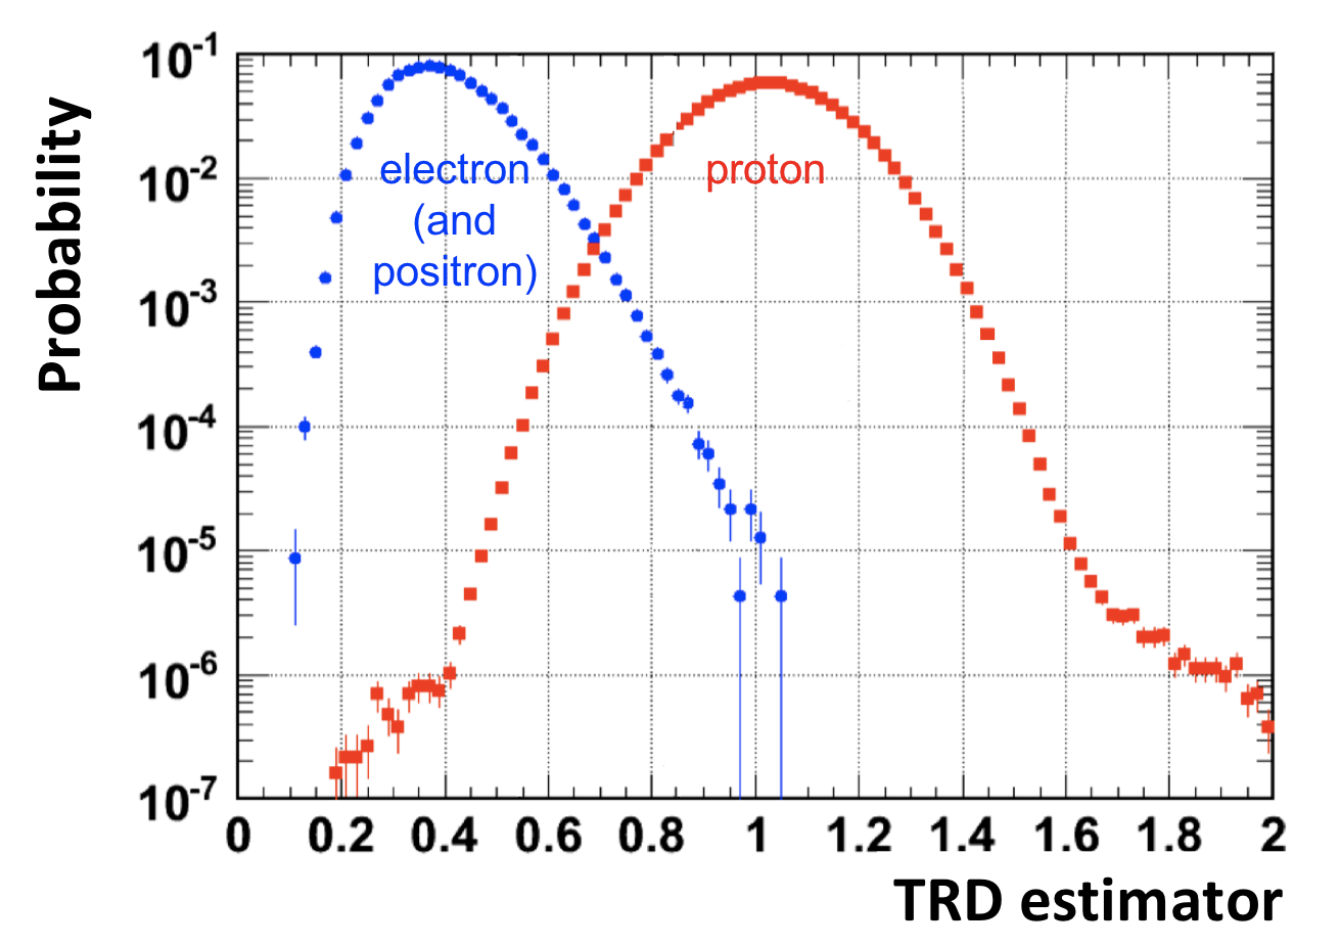
\includegraphics[width=0.80\textwidth]{Figures/chapter3/TRD/TRDEstimatorSeperation.png}
\includegraphics[width=1.00\textwidth]{Figures/chapter4/TRDLikelihood/{TRD_ChargeCorrectProtonTemplate_MC_B1042_pr.pl1.1800_7.6_all_Tree_positive_rigidity_14.1_15.3_pattern_0_bin_100_LogY_0.50}.pdf}
\caption[Seperation between the electrons and protons in $\Lambda_\mathrm{TRD}$ estimator.]{Seperation between the electrons and protons in $\Lambda_\mathrm{TRD}$ in the rigidity bin of 14.1 to 15.3 GV. The electrons and protons can be separated well in $\Lambda_\mathrm{TRD}$.}
\label{TRDEstimatorSeperation}
\end{figure}

the $\Lambda_\mathrm{TRD}$ provides separation power between electrons and protons. In figure \ref{TRDEstimatorSeperation}, the $\Lambda_\mathrm{TRD}$ is shown in the example rigidity bin of 14.1 to 15.3 GV, the electrons and protons can be distinguished well. At the 90\% electron efficiency range, the proton rejection power, which is defined as the inverse ratio of protons in this range, reaches more than $10^4$ \cite{TRDRejectionPowerPaper}. Similarly, the TRD likelihood estimator for the proton and the helium $\Lambda_{\mathrm{TRD}_{\mathrm{P/He}}}$ is defined as $-\rm{log}(\mathcal{L}_{p}/(\mathcal{L}_{p}+\mathcal{L}_{He}))$. \par


  

  
\section{Template Fit} \label{TempalteFitSection}

In this section, the template fits are shown in detail for the time-averaged analysis and the time-dependent analysis. The template fit is a method to extract signal and background events from the total event distribution. If the data distribution is $D(x)$ and it has $k$ components, then the goal of the template fit is to extract the event number of different components from the data distribution. In this analysis, the binned maximum likelihood fit is used. The fit is performed by minimizing the negative log-likelihood function $L$:

\begin{equation}
L = - \left ( \sum_{x}^{} D(x) \cdot {\rm{log}}(P(x)) - N_{{\rm{total}}} \right )
\end{equation}

where $N_{\rm{total}}$ is the total number of event, $P$ is the normalized likelihood, which is defined as the sum of the product of the number of events $N_{i}$ and the PDF of the template $P_i$:

\begin{equation}
P(x) = \sum_{i=1}^{k} N_{i} \cdot P_{i}(x)
\end{equation}

The minimization is achieved using the Minuit minimizer \cite{MinuitPaper}. The PDFs of templates are constructed before the template fit and the numbers of events are free parameters. By minimizing the negative log-likelihood function, the best-fit parameters, namely the number of events for signals and backgrounds, can be extracted.  \par

For different rigidity ranges, the template fit methods are different due to the sub-detector resolutions and background contributions. The selections used to obtain the signal and background templates will be discussed, and then the template fit result will be shown. In the time-dependent analysis, the template fit and the result in six Bartels Rotations will be given.   
 
%%%% Time averaged analysis
\subsection{Time-averaged analysis}
The first ingredient to construct the antiproton to proton flux ratio is the number of events. As the background levels can not be ignored, cut-based analysis is not enough to get clean signals. Therefore, in order to extract clean antiproton signals, the template fit method is used in this analysis. \par

In different rigidity ranges, the detector resolutions and background components are different, and the whole analysis is divided into three parts: low rigidity range (1.0 GV to 6.5 GV), intermediate rigidity range (3.0 to 19.5 GV), and high rigidity range (14.1 to 525 GV). The rigidity ranges are the same with the ones used in the previous AMS-02 antiproton analysis \cite{AMS02AntiprotonPRL2016}. In each range, a dedicated template fit method is used to get the antiproton signals, and the results in the overlappings from different template fit methods are used for crosschecks. \par

%% Low Range
\subsection*{Low Rigidity Range}
% 2D Template Fit method in TOF&TRD
In the low rigidity range, the dominant background sources are light particles. Except the electrons, the interaction between the incoming particles with the AMS-02 materials can produce secondary interaction particles like pions. These background components have to be separated from the antiproton signals. Since the particle's mass is calculated from rigidity and $\beta$ as given in equation \ref{MassEquation}, and the mass of the antiproton is much heavier than the background components in this range, the $\beta$ measurements of antiproton signal is different from the backgrounds in a specific rigidity bin. In this rigidity range, the TOF can be used to separate antiprotons and backgrounds by measuring the $\beta$. With the rigidity going up, the separation power from $\beta_{\rm{TOF}}$ decreases, and at the same time, the TRD separation power increases, so the $\Lambda_\mathrm{TRD}$ can take over afterwards in the intermediate rigidity range. A 2D template fit in $\Lambda_\mathrm{TRD}$ and $\beta_{\rm{TOF}}$ ($1/{\beta_{\rm{TOF}}}$) is used in the low rigidity range to have a smooth and stable separation power. The range in low rigidity is from 1.0 GV to 6.5 GV. The lower limit is due to the low statistics after the geometrical cutoff, and the higher limit is due to the $\beta_{\rm{TOF}}$ resolution. \par
% Templates
After the cuts and selections are applied, there are three major components in the data: antiprotons, electrons, and secondaries. The three templates must be constructed first to do the template fit. The antiproton template is taken from the ISS positive rigidity data since the clean proton data sample is easy to extract from it, and the rigidity sign does not impact the absolute value of the $\beta_{\rm{TOF}}$ and the $\Lambda_\mathrm{TRD}$. The electron and the secondaries templates are taken from the ISS negative rigidity data. To get the clean electron and secondaries samples from it, dedicated selections are applied for each sample respectively. Furthermore, after the preselection and selection introduced in Section \ref{DataSelectionSection}, the ISS data to be fitted should fulfill additional selection requirements in the low rigidity range. In table \ref{LowRigiditySelectionsForTemplates} the full list of selections is shown.  \par 

\begin{table}[h]
\setlength\tabcolsep{15pt}
\centering
\caption{List of selections to get all the templates and select further for the ISS data in the low rigidity range.} 
\label{LowRigiditySelectionsForTemplates}
\begin{tabular}{cc}
\hline \textbf{Antiproton Template}                                                                                                                             &  \textbf{Electron Template}                                                                                                                            \\
%\hline $\frac{1}{\beta_\mathrm{LowEdge}(R)} < \frac{1}{\beta_\mathrm{TOF}}-\frac{1}{\beta(R,m_{{\rm{p}}})}<0.2$    &  $\frac{1}{\beta_\mathrm{LowEdge}(R)}< \frac{1}{\beta_\mathrm{TOF}}-\frac{1}{\beta(R,m_{{\rm{p}}})}<0.2$  \\
%\hline $ \mathrm{\Lambda}_\mathrm{LowEdge}(R) < \Lambda_{\mathrm{TRD}} <  1.6 $                                                 &  $ \mathrm{\Lambda}_\mathrm{LowEdge}(R) < \Lambda_{\mathrm{TRD}} <  1.6 $                                                \\
\hline $ \Lambda_{\mathrm{TRD}_{\mathrm{P/He}}} < 0.1$                                                                                     &   Has $\beta$ measurement in RichAgl                                                                                                           \\
\hline TRD Number of tracks = 1                   &   | $ \beta_\mathrm{RICH} - \beta(R,m_{{\rm{e}}}) | <  0.002 $         \\
\hline TRD Number of hits < 40                     &   TRD Number of segments in XZ side = 1                                                     \\
\hline R > 0                                                    &   TRD Number of segments in YZ side = 1                                                     \\
\hline                                                              &   TRD Number of hits < 35                                                                             \\
\hline                                                              &    R < 0                                                                                                           \\
\hline       
\hline \textbf{Secondaries Template}                                                                   & \textbf{Further selections for ISS Data}               \\
%\hline $\frac{1}{\beta_\mathrm{LowEdge}(R)}< \frac{1}{\beta_\mathrm{TOF}}-\frac{1}{\beta(R,m_{{\rm{p}}})}<0.2$         & $\frac{1}{\beta_\mathrm{LowEdge}(R)}< \frac{1}{\beta_\mathrm{TOF}}-\frac{1}{ \beta(R,m_{{\rm{p}}}) }<0.2$  \\
%\hline $ \mathrm{\Lambda}_\mathrm{LowEdge}(R) < \Lambda_{\mathrm{TRD}} <  1.6 $                                                      & $ \mathrm{\Lambda}_\mathrm{LowEdge}(R) < \Lambda_{\mathrm{TRD}} <  1.6 $                                                \\
\hline Has $\beta$ measurement in RichAgl                                                                                                                 & $ \Lambda_{\mathrm{TRD}_{\mathrm{P/He}}} < 0.1$                                                                                     \\
\hline $ | \beta_\mathrm{RICH} - \beta(R,m_{{\rm{\pi}}}) | < 0.002 $   & TRD Number of segments in XZ = 1        \\
\hline TRD Number of segments in XZ side > 1                                                  & TRD Number of segments in YZ = 1       \\
\hline TRD Number of segments in YZ side > 1                                                  &  R < 0                                                       \\
\hline TRD Number of hits > 50                                                                           &                                                                  \\
\hline R < 0                                                                                                          &                                                                  \\  
\hline
\end{tabular}
\end{table}

%\begin{figure}[h]
%    \centering
%    \subfigure[]{
%        \includegraphics[width=0.51\textwidth, height=0.20\textheight ]{Figures/chapter4/TemplateFit/TimeAveragedPlot/Low/LowerEdge/{LowerEdge_TOF}.pdf} 
%    }\hspace{-0.9cm}
%    \subfigure[]{
%	\includegraphics[width=0.51\textwidth, height=0.20\textheight ]{Figures/chapter4/TemplateFit/TimeAveragedPlot/Low/LowerEdge/{LowerEdge_TRD}.pdf}
%    }
%    \caption[The rigidity dependence of a) 1/$\beta_{\rm{low}}$ and b) $\Lambda_{\mathrm{low}}$.]{The rigidity dependence of a) 1/$\beta_{\rm{LowEdge}}$ and b) $\Lambda_{\mathrm{LowEdge}}$ at the lower edge of the template fit range for 90\% signal efficiency. The red points correspond to the rigidity bin centers.}
%    \label{LowerEdgeOfLowTemplateFit}
%\end{figure}


In table \ref{LowRigiditySelectionsForTemplates}, $\beta_{\rm{RICH}}$ is the $\beta$ measurement from the RICH, $\beta(R,m)=\sqrt{\frac{R^2}{m^2+R^2}}$ is the $\beta$ value constructed with rigidity $R$ and mass $m$. Except for the cuts shown in the table, to remove most backgrounds before performing the template fit, additional template fit range cuts on $\beta_\mathrm{TOF}$ and $\Lambda_{\mathrm{TRD}}$ are applied to all the templates and ISS data to be fitted: $\frac{1}{\beta_\mathrm{LowEdge}(R)} < \frac{1}{\beta_\mathrm{TOF}}-\frac{1}{\beta(R,m_{{\rm{p}}})}<0.2$ and $ \mathrm{\Lambda}_\mathrm{LowEdge}(R) < \Lambda_{\mathrm{TRD}} <  1.6 $. $\beta_{\rm{LowEdge}}(R)$ and $\Lambda_{\mathrm{LowEdge}}(R)$ denote the low edge of the template fit range. By varying the low edges, the systematic uncertainty of the template fit can be evaluated. This will be discussed further later in Section \ref{SystematicUncertaintiesSection}. For the final time-averaged antiproton to proton flux ratio, the template fit result at 90\% signal efficiency is used. \par

%The rigidity dependence of $1/\beta_{\rm{LowEdge}}(R)$ and $\Lambda_{\mathrm{LowEdge}}(R)$ at the lower edge of the template fit range is shown in figure \ref{LowerEdgeOfLowTemplateFit}. \par

%Most cuts and selections are set using a fixed value except for the $1/\beta_{\rm{LowEdge}}(R)$ and $\Lambda_{\mathrm{LowEdge}}(R)$. These two cuts are the lower edge values of the template fit ranges and are rigidity-dependent. 
%$\beta(R,m_{{\rm{p}}})=\sqrt{\frac{R^2}{m_{{\rm{p}}}^2+R^2}}$ is the $\beta$ value constructed with rigidity and proton mass $m_{\rm{p}}$, 
%$\beta(R,m_{{\rm{e}}})=\sqrt{\frac{R^2}{m_{{\rm{e}}}^2+R^2}}$ is the $\beta$ value constructed with rigidity and electron mass $m_{\rm{e}}$, 
%$\beta(R,m_{{\rm{\pi}}})=\sqrt{\frac{R^2}{m_{{\rm{\pi}}}^2+R^2}}$ is the $\beta$ value constructed with rigidity and pion mass $m_{\rm{\pi}}$. \par


%%%%%%%%%%%%%%%%%%%%%%%%%%%%%%%%%%%%%%%%%%%%%%%%%%%
% Template Fit (Old)
%Once the templates are obtained, the template fit can be performed. In this analysis, the binned maximum likelihood fit is used. For example, in the low rigidity range, the likelihood function is written as:
%\begin{equation}
%f(\mathcal{L})=N_{\bar{p}} \cdot T_{\bar{p}}(\mathcal{L}) + N_{e^{-}} \cdot T_{e^{-}}(\mathcal{L}) + N_{s} \cdot T_{s}(\mathcal{L})
%\end{equation}
%where the $T_{\bar{p}}(\mathcal{L})$, $T_{e^{-}}(\mathcal{L})$ and $T_{s}(\mathcal{L})$ are the normalized antiproton, electron and secondaries templates respectively, and the $N_{\bar{p}}$, $N_{e^{-}}$ and $N_{s}$ are the free parameters in the fit, which are correspondent to the event numbers of these components. \par
%%%%%%%%%%%%%%%%%%%%%%%%%%%%%%%%%%%%%%%%%%%%%%%%%%%

\begin{figure}[htbp]
    \centering
    \subfigure[]{
         \includegraphics[width=1.0\textwidth,  trim=0.7cm 4.6cm 10cm 0.45cm, clip]{Figures/chapter4/TemplateFit/TimeAveragedPlot/Low/TemplateFit/fullrange/2DShowData/{FitResult_tof_2.97_3.29_pass7.8_TRDeff_1.00_TOFeff_1.00}.pdf} %xleftupper, yleftbottom, xrightbottom, yrightupper
         \label{LowRangeDataPlot}
    }
    \subfigure[]{
         \includegraphics[width=1.0\textwidth, trim=10.7cm 4.6cm 0 0.45cm, clip]{Figures/chapter4/TemplateFit/TimeAveragedPlot/Low/TemplateFit/fullrange/2DShowData/{FitResult_tof_2.97_3.29_pass7.8_TRDeff_1.00_TOFeff_1.00}.pdf}
         \label{LowRangeFitPlot}
    }
    \caption[Negative ISS data and Fit result in 2.97 to 3.29 GV]{a) Negative rigidity ISS data in the rigidity range of 2.97 to 3.29 GV in 1/$\beta_\mathrm{TOF}$ and $\Lambda_\mathrm{TRD}$ space. In the Y axis, 1/$\beta$ calculated with rigidity and antiproton mass is subtracted from the value of 1/$\beta_\mathrm{TOF}$, so the distribution of antiproton can be normalized to be around 0. Antiproton signal, electron and secondaries background components are seen in this plot. To remove the most backgrounds, $\Lambda_\mathrm{TRD}$ cut of 0.7 is applied in this plot. b) The 2D template fit result in the same rigidity bin of 2.97 to 3.29 GV in 1/$\beta_\mathrm{TOF}$ and $\Lambda_\mathrm{TRD}$ space.} 
\end{figure}


\begin{figure}[htbp]
    \centering
    \subfigure[]{
         \includegraphics[width=0.9\textwidth, height=0.43\textheight]{Figures/chapter4/TemplateFit/TimeAveragedPlot/Low/TemplateFit/fullrange/TOF-0.3TRD0.7/TOF-0.1TRD0.9/{1_TofBeta_Y_tof_LogY_2.97_3.29_pass7.8_TRDeff_1.00_TOFeff_1.00}.pdf}
    }
    \vspace{-0.2cm}
    \par 
    \subfigure[]{
	\includegraphics[width=0.9\textwidth, height=0.43\textheight]{Figures/chapter4/TemplateFit/TimeAveragedPlot/Low/TemplateFit/fullrange/TOF-0.3TRD0.7/TOF-0.1TRD0.9/{TrdLikelihood_X_tof_LogY_2.97_3.29_pass7.8_TRDeff_1.00_TOFeff_1.00}.pdf}	
    }
    \caption[Example template fit in the low rigidity range of 2.97 to 3.29 GV.]{Example template fit in the low rigidity range of 2.97 to 3.29 GV. a) 1/$\beta_\mathrm{TOF}$ projection. In this projection, 1/$\beta$ calculated with rigidity and antiproton mass is subtracted from the value of 1/$\beta_\mathrm{TOF}$. b) $\Lambda_\mathrm{TRD}$ projection.}
    \label{LowRigidityExampleTemplateFitProjections}
\end{figure}

In figure \ref{LowRangeDataPlot}, the negative rigidity ISS data in the rigidity range of 2.97 to 3.29 GV is shown in 1/$\beta_\mathrm{TOF}$ and $\Lambda_\mathrm{TRD}$ space. The three components are antiprotons, electrons and interaction secondaries. $\Lambda_\mathrm{TRD}$ cut of 0.7 is applied in this plot to remove the most backgrounds of electrons and interaction secondaries. In figure \ref{LowRangeFitPlot}, an example template fit in this rigidity range is shown. To illustrate the separation, the 2D template fit is shown in two projections in figure \ref{LowRigidityExampleTemplateFitProjections}. In 1/$\beta_\mathrm{TOF}$ projection, further cut of $\Lambda_{\rm{TRD}}>0.9$ is applied to reduce the backgrounds; similarly in $\Lambda_\mathrm{TRD}$ projection, further cut of 1/$\beta_\mathrm{TOF}$-1/$\beta(R,m_{p})$>-0.1 is applied. Since it is a 2D template fit, the $\chi^2$/ndf is calculated individually in the two projections. \par

The template fits give the number of antiproton events in the low rigidity range. The proton number is obtained after selections introduced in Section \ref{DataSelectionSection} and further selections for ISS data in table \ref{LowRigiditySelectionsForTemplates} but $R>0$. In figure \ref{PbarNumbersInLowRigidityRange} the number of antiproton and proton events as a function of the rigidity obtained is given. 
%The corresponding $\chi^2$/ndf values of the template fits are given in figure \ref{Chi2OfFitInLowRigidityRange}.  \par

\begin{figure}[H]
\includegraphics[width=1.00\textwidth]{Figures/chapter4/TemplateFit/TimeAveragedPlot/Low/{NumberPbarAndProtonPlot_LowRange_pass78}.pdf}
\caption[The number of antiproton and proton events obtained in the low rigidity range.]{The numbers of antiproton and proton events as function of the rigidity obtained in the low rigidity range.}
\label{PbarNumbersInLowRigidityRange}
\end{figure}

%\begin{figure}[H]
%\includegraphics[width=1.00\textwidth]{Figures/chapter4/TemplateFit/TimeAveragedPlot/Low/FitResult/{chi2_tof_pass7.8_TRDEff_0.94_TOFEff_0.95}.pdf}
%\caption{The $\chi^2$/ndf of the template fits in the low rigidity range.}
%\label{Chi2OfFitInLowRigidityRange}
%\end{figure}


%% Intermediate Range
\subsection*{Intermediate Rigidity Range}
% Template Fit method in TRD
In the intermediate rigidity range, the 2D template fit in $\beta_{\rm{TOF}}$ and $\Lambda_\mathrm{TRD}$ is replaced by a 1D template fit in $\Lambda_\mathrm{TRD}$ since the separation power of $\beta_{\rm{TOF}}$ decreases with the rigidity going up and provides little power in this rigidity range. Above 20 GV, the component of charge confused protons gradually increases, so it has to be added as an additional template. Therefore the 1D template fit can only be implemented up to around 20 GV. \par

% Templates
In the intermediate rigidity range, the interaction secondaries component is negligible. Therefore, the templates in this rigidity range are only formed for antiprotons and electrons. Like the template fit in the low rigidity range, the templates are also taken from the ISS data. The antiproton template is taken from positive rigidity data, and the electron template is taken from negative rigidity data. The dedicated selections for ISS data in the intermediate rigidity range are applied before the template fit. In table \ref{IntermediateRigiditySelectionsForTemplates}, the full list of selections that are used for the ISS data and in order to form the templates is given.  \par

\begin{table}[htbp]
\setlength\tabcolsep{15pt}
\centering
\caption{List of selections to get all the templates and select further for the ISS data in the intermediate rigidity range.} 
\label{IntermediateRigiditySelectionsForTemplates}
\begin{tabular}{cc}
\hline \textbf{Antiproton Template}      &  \textbf{Electron Template}           \\
%\hline PatternCut                             &  PatternCut                                    \\
%\hline $ \mathrm{\Lambda}_\mathrm{LowEdge}(R) < \Lambda_{\mathrm{TRD}} < 2 $  &  $ \mathrm{\Lambda}_\mathrm{LowEdge}(R) < \Lambda_{\mathrm{TRD}} < 2 $  \\
\hline $\beta_\mathrm{RICH}<\beta_\mathrm{high}(R)$                                             &   TRD Number of hits < 35                          \\
\hline TRD Number of segments in XZ side = 1                                                                  &   ECALBDT > 0.5                                         \\
\hline TRD Number of segments in YZ side = 1                                                                  &   TRD Number of segments in XZ side = 1         \\
\hline R > 0                                                                                                                   &   TRD Number of segments in YZ side = 1        \\
\hline                                                                                                                            & R < 0                                                           \\
%\hline                                                                                                                         &  $TRDLogLikelihood>-1.5$                         \\
\hline \textbf{Further selections for ISS Data}                                                                            &        \\
%\hline PatternCut                                                                                                      &        \\
%\hline  $ \mathrm{\Lambda}_\mathrm{LowEdge}(R) < \Lambda_{\mathrm{TRD}} < 2 $ &        \\
\hline  $\beta_\mathrm{RICH}<\beta_\mathrm{high}(R)$                                            &        \\
\hline  TRD Number of segments in XZ side = 1                                                                 &        \\
\hline  TRD Number of segments in YZ side = 1                                                                  &        \\
\hline  R < 0                                                                                                                   &        \\
\hline
\end{tabular}
\end{table}

\begin{figure}[htbp]
\centering
%\includegraphics[width=1.00\textwidth]{Figures/chapter4/TemplateFit/TimeAveragedPlot/intermediate/TemplateFit/{FitResult_0124_free_pass7.8_10.1_11_TRDEff_0.90}.pdf}
\includegraphics[width=1.00\textwidth]{Figures/chapter4/TemplateFit/TimeAveragedPlot/intermediate/TemplateFit_FullRange/{FitResult_LogY_0124_free_pass7.8_5.9_6.47_TRDEff_1.00}.pdf}
%\caption{Example template fit in the intermediate rigidity range of 10.1 to 11.0 GV.}
\caption[Example template fit in the intermediate rigidity range of 5.9 to 6.47 GV.]{Example template fit in the intermediate rigidity range of 5.9 to 6.47 GV. To reduce the most electrons, the template fit is performed on the right side of the dashed line, which corresponds to around 99\% antiproton signal efficiency.}
\label{ExampleTemplateFitInIntermediateRange}
\end{figure}

In table \ref{IntermediateRigiditySelectionsForTemplates}, the ECALBDT estimator is a value trained with ECAL response variables and can provide separation power between protons and electrons. If the particles go through the ECAL, a clean electron sample can be obtained by applying a cut of 0.5 on ECALBDT. To avoid the light particles background, if there is a $\beta_{\rm{RICH}}$ measurement then the value has to be less than $\beta_\mathrm{high}(R)$ to restrict the signal range. The $\beta_\mathrm{high}(R)$ is determined by 90\% antiproton signal efficiency. Except for the cuts in this table, to remove most backgrounds before performing the template fit, an additional template fit range cut on $\Lambda_{\mathrm{TRD}}$ is applied to all the templates and ISS data to be fitted like described in the low rigidity range.  \par 


% Example Fit
In figure \ref{ExampleTemplateFitInIntermediateRange}, an example template fit in the rigidity range of 5.9 to 6.47 GV is shown. The antiproton signal can be separated well from the electron background. To reduce the most background of electrons, the template fit range is set to around 99\% antiproton signal efficiency (the dashed line).

The template fits give the number of antiproton events in the intermediate rigidity range. The proton number is obtained after selections introduced in Section \ref{DataSelectionSection} and further selections for ISS data in table \ref{IntermediateRigiditySelectionsForTemplates} but $R>0$. The obtained antiproton and proton numbers are shown in figure \ref{PbarNumbersInIntermediateRigidityRange}. 
%The corresponding $\chi^2$/ndf values of the template fits in the intermediate rigidity range are given in Figure \ref{Chi2OfFitInIntermediateRigidityRange}. \par

\begin{figure}[H]
\includegraphics[width=1.00\textwidth]{Figures/chapter4/TemplateFit/TimeAveragedPlot/intermediate/{NumberPbarAndProtonPlot_IntermediateRange_pass78}.pdf}
\caption[The number of antiproton and proton events obtained in the intermediate rigidity range.]{The numbers of antiproton and proton events as function of the rigidity obtained in the intermediate rigidity range.}
\label{PbarNumbersInIntermediateRigidityRange}
\end{figure}

%\begin{figure}[t]
%\includegraphics[width=1.00\textwidth]{Figures/chapter4/TemplateFit/TimeAveragedPlot/intermediate/TemplateFit/{chi2dof_0124_free_pass7.8binmerge1_TRDEff_0.90}.pdf}
%\caption{The $\chi^2$/ndf of the template fits in the intermediate rigidity range.}
%\label{Chi2OfFitInIntermediateRigidityRange}
%\end{figure}

%% High Range
\subsection*{High Rigidity Range}

% Template Fit method in CC vs. TRD
In the high rigidity range, the contribution of charge confused protons increases. Therefore, the $\Lambda_{\rm{CC}}$ trained in Section \ref{chargeconfusion} is used to separate antiprotons and charge confused protons. For electron separation, the TRD provides separation power, like in the low and intermediate rigidity ranges. In summary, a 2D template fit in $\Lambda_{\rm{CC}}$ and $\Lambda_\mathrm{TRD}$ is performed in this range to get the antiproton signal. \par

\begin{figure}[tph]
    \centering
    
    \subfigure[]{
         \includegraphics[width=0.90\textwidth,  trim=0.5cm 7.5cm 10cm 0.7cm, clip]{Figures/chapter4/TemplateFit/TimeAveragedPlot/high/TemplateFit/{FitResult_Pattern_0_VGG16NN_175_211_cccut_0.20_CCN_20_TRDN_20}.pdf} %xleftupper, yleftbottom, xrightbottom, yrightupper
         \label{HighRangeDataPlot} 
    }
    \vspace{-0.2cm}
    \par
    \subfigure[]{
         \includegraphics[width=0.9\textwidth, trim=10.5cm 7.5cm 0 0.7cm, clip]{Figures/chapter4/TemplateFit/TimeAveragedPlot/high/TemplateFit/{FitResult_Pattern_0_VGG16NN_175_211_cccut_0.20_CCN_20_TRDN_20}.pdf}
         \label{HighRangeFitPlot}
    }
    \caption[Negative rigidity ISS data and fit result in the rigidity range of 175 to 211 GV in $\Lambda_{\rm{CC}}$ and $\Lambda_\mathrm{TRD}$ space.]{a) Negative rigidity ISS data in the rigidity range of 175 to 211 GV in $\Lambda_{\rm{CC}}$ and $\Lambda_\mathrm{TRD}$ space. Three components of antiprotons, electrons and charge confused protons are seen in this plot. To remove most backgrounds of charge confused protons, $\Lambda_{\rm{CC}}$ cut of 0.2 is applied. b) The 2D template fit result in the same rigidity bin of 175 to 211 GV in $\Lambda_{\rm{CC}}$ and $\Lambda_\mathrm{TRD}$ space.}    
\end{figure}


\begin{figure}[htbp]
    \centering
    \subfigure[]{
        \includegraphics[width=0.9\textwidth, height=0.43\textheight]{Figures/chapter4/TemplateFit/TimeAveragedPlot/high/TemplateFit/{CCprojection_Pattern_0_VGG16NN_175_211_cccut_0.20_CCN_20_TRDN_20}.pdf} 
    }
     \vspace{-0.2cm}
    \par
    \subfigure[]{
	\includegraphics[width=0.9\textwidth, height=0.43\textheight]{Figures/chapter4/TemplateFit/TimeAveragedPlot/high/TemplateFit/{TRDprojection_Pattern_0_VGG16NN_175_211_cccut_0.20_CCN_20_TRDN_20}.pdf} 
    }
    \caption[Example template fit in the high rigidity range of 175 to 211 GV.]{Example template fit in the high rigidity range of 175 to 211 GV. a) In the $\Lambda_{\rm{CC}}$ projection, $\Lambda_{\rm{TRD}}$>0.7 is applied and antiproton and charge confused proton can be separated well in this projection.  b) In the $\Lambda_\mathrm{TRD}$ projection, $\Lambda_{\rm{CC}}$>0.75 is applied and antiproton and electron can be separated well.}
    \label{ExampleTemplateFitInHighRigidityRange}
\end{figure}

% Tracker Pattern usage in Rigidity ranges 
As shown in figure \ref{TrackerResolutions}, different tracker patterns have different rigidity resolutions. To maximize the statistics and maintain the accuracy of rigidity measurement, the requirement of tracker patterns changes as rigidity goes up: No hit in tracker layers 1 and 9 is required below 38.9 GV; hit in either layer 1 and 9 is required from 38.9 to 147 GV; hit in layer 9 is required from 147 to 175 GV. Above 175 GV, hits in layers 1 and 9 are required. This selection requirement is the same as the one used in the previous AMS-02 publication \cite{AMS02AntiprotonPRL2016}. From 80.5 GV, every two rigidity bins are merged to increase the statistics. \par

% Templates
In the 2D template fit, the three templates are antiprotons, electrons, and charge confused protons. The antiproton template is taken from the ISS positive rigidity data, and the electron template is taken from the ISS negative rigidity data by ECALBDT. Finally, the charge confused proton template is formed by using proton MC simulation samples by selecting events with negative rigidity. To avoid the contamination of helium, the $\Lambda_{\mathrm{TRD}_{\mathrm{P/He}}} < 0.3$ cut is applied for the negative rigidity data before the template fit. \par      %%--trd low 0.0 --trd high 1.6
%the electron template is taken from the ISS negative rigidity data by ECALBDT to be larger than zero

% Table of selection (Commented Out)
\begin{comment}
\begin{table}[h]
\setlength\tabcolsep{15pt}
\centering
\caption{List of selections for templates}
\label{HighRigiditySelectionsForTemplates}
\begin{tabular}{cc}
\hline \textbf{Antiproton template}                         &  \textbf{Electron Template}                         \\
\hline         $-1<ECALBDT<0$                                 &  $0<ECALBDT$                                       \\
\hline         $\rm{TRDLikelihood_{P/He}} < 0.3$      &   $\rm{TRDLikelihood_{P/He}} < 0.3$      \\
\hline \textbf{Charge confused proton Template}  &  \textbf{Negative Rigidity Data}                  \\
\hline         $-1<ECALBDT<0$                                 &   $-2<ECALBDT<0$                                 \\
\hline         $\rm{TRDLikelihood_{P/He}} < 0.3$,     &   $\rm{TRDLikelihood_{P/He}} < 0.3$      \\
\hline
\end{tabular}
\end{table}
\end{comment}

% Example Fit
To cut away the most background of charge confused protons, the template fit is performed in $\Lambda_{\rm{CC}}>0.2$ range. In figure \ref{HighRangeDataPlot}, the negative rigidity ISS data in the rigidity range of 175 to 211 GV is shown in $\Lambda_{\rm{CC}}$ and $\Lambda_\mathrm{TRD}$ space. The three components of antiprotons, electrons and charge confused protons are indicated in this figure. In figure \ref{HighRangeFitPlot}, an example template fit in this rigidity range is shown. To illustrate the separation, the 2D template fit is shown in two projections in figure \ref{ExampleTemplateFitInHighRigidityRange}. In $\Lambda_{\rm{CC}}$ projection, $\Lambda_{\rm{TRD}}$>0.7 is applied to show the separation between antiprotons and charge confused protons. In $\Lambda_\mathrm{TRD}$ projection, $\Lambda_{\rm{CC}}$>0.75 is applied to show the separation between antiprotons and electrons. Since it is a 2D template fit, the $\chi^2$/ndf is calculated individually in the two projections. \par
%In $\Lambda_{\rm{CC}}$ projection, further cut of $\Lambda_{\rm{TRD}}>0.5$ is applied to show the separation between antiprotons and charge confused protons. In $\Lambda_\mathrm{TRD}$ projection, further cut of  $\Lambda_{\rm{CC}}>0.4$ is applied to show the separation between antiprotons and electrons. \par

%The number of antiprotons obtained from the 2D template fit and the number of protons after the selections introduced in Section \ref{DataSelectionSection} are given in figure \ref{PbarNumbersInHighRigidityRange}.  
The numbers of antiprotons and protons obtained in the high rigidity range are given in figure \ref{PbarNumbersInHighRigidityRange}.  


%For example, the corresponding $\chi^2$/ndf in the full span is given in \ref{Chi2OfFitInHighRigidityRange}. \par 

\begin{figure}[hptb]
\includegraphics[width=1.00\textwidth]{Figures/chapter4/TemplateFit/TimeAveragedPlot/high/{NumberPlot_AllPatternsOverRigidityBinWidthpass78}.pdf}
\caption[The antiproton and proton numbers obtained in the high rigidity range.]{The antiproton and proton numbers obtained in the high rigidity range. The dashed vertical lines are the boundary of the usage of different tracker patterns. To avoid the jump due to the merge of rigidity bins from 80.5 GV, the antiproton and proton numbers are divided by the rigidity bin width to have a smooth curve.}
\label{PbarNumbersInHighRigidityRange}
\end{figure}

Once the template fits in the three rigidity ranges are performed, the antiproton numbers from 1.0 to 525 GV can be obtained. In total, 481959 antiprotons are selected from the template fits. \par

%\begin{figure}[H]
%\includegraphics[width=1.00\textwidth]{Figures/chapter4/TemplateFit/TimeAveragedPlot/high/FitResult/{Chi2dof_Pattern_0_pass7.8_VGG16NN}.pdf}
%\caption{The $\chi^2$/ndf of template fit in full span in the high rigidity range.}
%\label{Chi2OfFitInHighRigidityRange}
%\end{figure}



%In figure \ref{PbarTimeAveragedNumbers}, the antiproton number plot is shown. 
%\begin{figure}[H]
%\centering
%\includegraphics[width=1.00\textwidth]{Figures/chapter4/TemplateFit/TimeAveragedPlot/{NumberPlot_pass78_AllRange}.pdf}
%\caption{The antiproton numbers get from the template fit result.}
%\label{PbarTimeAveragedNumbers}
%\end{figure}


%%%% Time-dependent analysis
\subsection{Time-dependent analysis}

% Template Fit method
For the time-dependent analysis, the template fit strategy is the same as the one used in the time-averaged analysis. The data is divided into time bins with a width equal to the duration of six Bartels Rotations each. In each time bin, a template fit is performed to get the antiproton to proton ratio. Due to the limited statistics in each time bin, the rigidity binning is altered in the following way: every two original neighboring rigidity bins are now merged to form a new bin. In this way, an increase in statistics in each new bin is accomplished. \par

% Time Dependent Template
The template selections are the same as the ones used in the time-averaged analysis. The only difference is the template fit range. To increase the statistics, the signal efficiency is increased from 90\% to 95\% in the low rigidity range and from 90\% to 98\% in the intermediate rigidity range. \par

Since the templates are taken from the ISS data, the shapes of the templates are time-dependent. To visualize the time dependence, all the templates are parameterized in the distribution core range in the following way: In the $\Lambda_\mathrm{TRD}$ dimension, the antiproton, electron and secondaries are parameterized by a Novosibirsk function $N(x;\mu,\sigma,\tau)$, and in the 1/$\beta_\mathrm{TOF}$ dimension, the antiproton, electron and secondaries are parameterized by a Gaussian function $G(x; \mu,\sigma)$: \par

\begin{figure}[hptb]
\centering
\includegraphics[width=1.00\textwidth]{Figures/chapter4/TemplateFit/TimeDependentPlot/TimeDependentTemplate/TRD/{TemplateFit_TRD_6.47_7.76_78}.pdf}
\caption[The parameterizations of the normalized antiproton and electron templates.]{The parameterizations of the normalized antiproton and electron templates by Novosibirsk functions in the rigidity range of 6.47 to 7.76 GV with data collected from Feb.18.2017 to Jul.30.2017.}
\label{PparameterizationsTemplate}
\end{figure}

\begin{equation}
\begin{aligned}
G(x; \mu,\sigma) &= \frac{1}{\sqrt{2 \pi \sigma^2}}{\rm{exp}} \left(-\frac{(x-\mu)^2}{2\sigma^2} \right), \\
N(x;\mu,\sigma,\tau)&={\rm{exp}}\left( -\frac{1}{2} \left( \frac{({\rm{ln}}(\lambda(x; \mu,\sigma,\tau)))^2}{\tau^2}+\tau^2  \right)  \right), {\rm{where}}\\
\lambda(x; \mu,\sigma,\tau)&=1+\tau(x-\mu)\frac{{\rm{sinh}}(\tau\sqrt{{\rm{ln}}4})}{\sigma\tau\sqrt{{\rm{ln}}4}}
\end{aligned}
\end{equation}

% TRD side:
For an illustration of parameterization in the $\Lambda_\mathrm{TRD}$ dimension, the parameterizations of the normalized antiproton and electron templates in the rigidity range of 6.47 to 7.76 GV with data collected from Feb.18.2017 to Jul.30.2017 is shown as an example in figure \ref{PparameterizationsTemplate}. 

\begin{figure}[hptb]
    \centering
    \subfigure[]{
        \includegraphics[width=0.49\textwidth, height=0.23\textheight]{Figures/chapter4/TemplateFit/TimeDependentPlot/TimeDependentTemplate/TRD/Antiproton/{Antiproton_TRD_6.47_7.76_miu}.pdf} 
    }
    \hspace{-0.7cm}
    \subfigure[]{
	\includegraphics[width=0.49\textwidth, height=0.23\textheight]{Figures/chapter4/TemplateFit/TimeDependentPlot/TimeDependentTemplate/TRD/Antiproton/{Antiproton_TRD6.47_7.76_sigma}.pdf} 
    } 
    \subfigure[]{
        \includegraphics[width=0.49\textwidth, height=0.23\textheight]{Figures/chapter4/TemplateFit/TimeDependentPlot/TimeDependentTemplate/TRD/Electron/{Electron_TRD_6.47_7.76_miu}.pdf} 
    } 
    \hspace{-0.7cm}
    \subfigure[]{
	\includegraphics[width=0.49\textwidth, height=0.23\textheight]{Figures/chapter4/TemplateFit/TimeDependentPlot/TimeDependentTemplate/TRD/Electron/{Electron_TRD6.47_7.76_sigma}.pdf} 
    }
    %\vspace{-10mm}        
    \caption[Time-dependence of the a) $\mu_{\rm{\bar{p},TRD}}$ b) $\sigma_{\rm{\bar{p},TRD}}$ c) $\mu_{\rm{e^{-},TRD}}$ d) $\sigma_{\rm{e^{-},TRD}}$ in 6.47 to 7.76 GV.]{Time-dependence of the a) $\mu_{\rm{\bar{p},TRD}}$ b) $\sigma_{\rm{\bar{p},TRD}}$ c) $\mu_{\rm{e^{-},TRD}}$ d) $\sigma_{\rm{e^{-},TRD}}$ in the rigidity range of 6.47 to 7.76 GV. The parameters of the electron template show significant structures up to the end of 2012, where the TRD gas parameters were being optimized. After that, both parameters of antiproton and electron templates are changing due to the decrease of the Xe partial pressure in the TRD.}
    \label{TimeDependenceParameters}
\end{figure}

\begin{figure}[htbp]
    \centering
    \subfigure[]{
        \includegraphics[width=0.49\textwidth, height=0.23\textheight]{Figures/chapter4/TemplateFit/TimeDependentPlot/TimeDependentTemplate/TOF/Antiproton/{Antiproton_TOF_3.64_4.43_miu}.pdf} 
    }
    \hspace{-0.7cm}
    \subfigure[]{
	\includegraphics[width=0.49\textwidth, height=0.23\textheight]{Figures/chapter4/TemplateFit/TimeDependentPlot/TimeDependentTemplate/TOF/Antiproton/{Antiproton_TOF3.64_4.43_sigma}.pdf} 
    } 
    \subfigure[]{
        \includegraphics[width=0.49\textwidth, height=0.23\textheight]{Figures/chapter4/TemplateFit/TimeDependentPlot/TimeDependentTemplate/TOF/Electron/{Electron_TOF_3.64_4.43_miu}.pdf} 
    } 
    \hspace{-0.7cm}
    \subfigure[]{
	\includegraphics[width=0.49\textwidth, height=0.23\textheight]{Figures/chapter4/TemplateFit/TimeDependentPlot/TimeDependentTemplate/TOF/Electron/{Electron_TOF3.64_4.43_sigma}.pdf} 
    }  
    \subfigure[]{
        \includegraphics[width=0.49\textwidth, height=0.23\textheight]{Figures/chapter4/TemplateFit/TimeDependentPlot/TimeDependentTemplate/TOF/Pion/{Pion_TOF_3.64_4.43_miu}.pdf} 
    } 
    \hspace{-0.7cm}
    \subfigure[]{
	\includegraphics[width=0.49\textwidth, height=0.23\textheight]{Figures/chapter4/TemplateFit/TimeDependentPlot/TimeDependentTemplate/TOF/Pion/{Pion_TOF3.64_4.43_sigma}.pdf}  
    }
    \caption[Time-dependence of the a) $\mu_{\rm{\bar{p}},TOF}$ b) $\sigma_{\rm{\bar{p}},TOF}$ c) $\mu_{\rm{e^{-}},TOF}$ d) $\sigma_{\rm{e^{-}},TOF}$ e) $\mu_{\rm{secondaries},TOF}$ f) $\sigma_{\rm{secondaries},TOF}$ in 3.64 to 4.43 GV.]{Time-dependence of the a) $\mu_{\rm{\bar{p}},TOF}$ b) $\sigma_{\rm{\bar{p}},TOF}$ c) $\mu_{\rm{e^{-}},TOF}$ d) $\sigma_{\rm{e^{-}},TOF}$ e) $\mu_{\rm{secondaries},TOF}$ f) $\sigma_{\rm{secondaries},TOF}$ in the rigidity range of 3.64 to 4.43 GV. No obvious trend is observed in the mean values but the distributions of sigma show rising trends in all three components, this could be due to the aging of the scintillators.}
    \label{TimeDependenceTOFPara}
\end{figure}


For the antiproton template, the time dependence can be described by the mean value $\mu_{\rm{\bar{p},TRD}}$ and width $\sigma_{\rm{\bar{p}},TRD}$. For the electron template, the time dependence can be described by the mean value $\mu_{\rm{e^{-}},TRD}$ and width $\sigma_{\rm{e^{-}},TRD}$. The time dependence of the four parameters in the rigidity range of 6.47 to 7.76 GV is shown in figure \ref{TimeDependenceParameters}.


% TOF side:
%For an illustration of parameterization in the 1/$\beta_\mathrm{TOF}$ dimension, the parameterizations of the normalized antiproton, electron and secondaries templates in the rigidity range of X.XX to X.XX GV with data collected from Feb.18.2017 to Jul.30.2017 is shown as an example in figure \ref{XXX}.

For the 1/$\beta_\mathrm{TOF}$ dimension, the cores of the normalized antiproton, electron and secondaries templates are parametrized by Gaussian functions. The time dependence of the antiproton template can be described by the mean value $\mu_{\rm{\bar{p}},TOF}$ and width $\sigma_{\rm{\bar{p}},TOF}$, the time dependence of the electron template can be described by the mean value $\mu_{\rm{e^{-}},TOF}$ and width $\sigma_{\rm{e^{-}},TOF}$, the time dependence of the secondaries can be described by the mean value $\mu_{\rm{secondaries},TOF}$ and width $\sigma_{\rm{secondaries},TOF}$. The six parameters in an example rigidity range of 3.64 to 4.43 GV are shown in figure \ref{TimeDependenceTOFPara}.\par



% Example Template Fit
An example template fit in the rigidity range of 6.47 to 7.76 GV is given in figure \ref{TimeDependentTemplateFitInInermediate}. The fitted data is six Bartels Rotations data taken from Feb.18.2017 to Jul.30.2017. \par

\begin{figure}[htpb]
\centering
%\includegraphics[width=1.00\textwidth]{Figures/chapter4/TemplateFit/TimeDependentPlot/intermediate/FitPlot/{FitResult_0124_free_6.47_7.76_index_114_LogY}.pdf}
%\caption{Example template fit in the rigidity range of 6.47 to 7.76 GV with data collected from Jan.07.2020 to June.17.2020.}  % 1578355200 to 1592352000
\includegraphics[width=1.00\textwidth]{Figures/chapter4/TemplateFit/TimeDependentPlot/intermediate/FitPlot_FullRange/{FitResult_0124_free_6.47_7.76_index_78_TRDEff_1.00_LogY}.pdf}
\caption[Example template fit in 6.47 to 7.76 GV with data from Feb.2017 to Jul.2017.]{Example template fit in the rigidity range of 6.47 to 7.76 GV with data collected from Feb.18.2017 to Jul.30.2017.}  % 1494374400 to 1508371200
%To collect the most statistics of antiproton signal, no cut on the $\Lambda_\mathrm{TRD}$ is applied.
\label{TimeDependentTemplateFitInInermediate}
\end{figure}

The obtained antiproton numbers in 6.47 to 7.76 GV for the 23 groups containing data of six Bartels Rotations each is shown in figure \ref{PbarNumbersInTimeDependentIntermediateRange}. The corresponding values of the $\chi^2$/ndf are given in figure \ref{Chi2dofOfTimeDependentIntermediateRange}.  

\begin{figure}[htpb]
\centering
\includegraphics[width=1.00\textwidth, height=0.4\textheight]{Figures/chapter4/TemplateFit/TimeDependentPlot/intermediate/FitResult/{AntiprotonNumber_6BartalRotation_0124_free_binmerge2_6.47_7.76}.pdf}
\caption[Antiproton numbers in 6.47 to 7.76 GV with six Bartels' Rotation.]{The antiproton numbers obtained from the template fit results in the rigidity range of 6.47 to 7.76 GV with six Bartels' Rotation time resolution. To avoid jumps due to the measuring time (see Section \ref{MeasuringTimeSection}), the numbers are divided by the measuring time in each six Bartels' Rotation time bin.}
\label{PbarNumbersInTimeDependentIntermediateRange}
\end{figure}

\begin{figure}[htpb]
\centering
\includegraphics[width=1.00\textwidth, height=0.4\textheight]{Figures/chapter4/TemplateFit/TimeDependentPlot/intermediate/FitResult/{Chi2dof_6BartalRotation_0124_free_binmerge2_6.47_7.76}.pdf}
\caption[$\chi^2$/ndf of the fits in 6.47 to 7.76 GV with six Bartel's Rotation.]{$\chi^2$/ndf of the template fits in the rigidity range of 6.47 to 7.76 GV with six Bartel's Rotation time resolution.}
\label{Chi2dofOfTimeDependentIntermediateRange}
\end{figure}




%\subsection*{Low Rigidity Range}
% Template Fit method 
%In the low rigidity range, the 2D template fit in TRDLikelihood vs. TOF beta is performed from 1.16 to 6.47 GV.  \par
% Templates
% TOFBetaCut和TrdLikelihoodCut 是在fit时候补上了边界的。
% Pabr      : PositiveCut(TRD_{low}<TrdLikelihoodCut && TrdLikelihoodHeProton<0.1 && TRDVTracksSize=1 && TrdNumberOfHitsCut_P<40; )  %比averaged少了TOFBetaCut
% Electron: ElectronTemplateDataCut ("RichIsNaF==0 && RichBeta-(-Rigidity)/sqrt(0.000511^2+Rigidity^2)>-0.002 && TrdSegmentsXZNumber==1 && TrdSegmentsYZNumber==1 && TrdNumberOfHits<35")  %比averaged少了TOFBetaCut 和 TRDLikelihoodCut
% Pion      : PionTemplateDataCut (  (std::string("RichIsNaF==0 && abs(RichBeta-(-Rigidity)/sqrt(0.139^2+Rigidity^2))<0.002 && TrdLogLikelihoodRatioElectronProtonTracker>") + std::to_string(TrdLOW) + std::string("&& TrdSegmentsXZNumber>1 && TrdSegmentsYZNumber>1 && TrdNumberOfHits>50")).c_str(); )    %比averaged少了TOFBetaCut
% Data      : NegativeCut   ( TrdLikelihoodCut && TrdLikelihoodHeProtonCut && TrdSegmentsXZNumberCut && TrdSegmentsYZNumberCut;) 
% Example Fit



%\subsection*{Intermediate Rigidity Range}
% Template Fit method 
% Templates
% Example Fit


  


\section{Effective Acceptance} \label{EffectiveAcceptanceSection}

%% Definition 
After the event number is determined by the template fit, the next important ingredient to calculate the antiproton to proton flux ratio is the effective acceptance.    \par

For a spectrometer, the counting rate of a given particle species depends on the flux intensity and the geometrical acceptance $A_\mathrm{geo}$ \cite{SULLIVAN19715}. The geometrical acceptance is a fixed value for a certain apparatus, but this assumes no interaction between the traversing particles and the apparatus, while for data analysis, dedicated cuts and selections are applied. Therefore, considering this, the geometrical acceptance is multiplied by the efficiencies of the cuts and the selections $\epsilon_\mathrm{cut}$. This product is called effective acceptance $A_\mathrm{eff}$. The larger the effective acceptance, the more events can be collected. \par

\begin{equation}
\label{EffectiveAcceptanceDefination}
A_\mathrm{eff}=A_\mathrm{geo} \times \epsilon_\mathrm{cut} 
\end{equation}

%% Calculating acceptance: Acceptance in AMS-02
Calculating the effective acceptance directly is impossible. The practical way is to use the MC simulation method. In the AMS-02 experiment, different MC production models with the help of Geant4 are widely used. In these models, the whole detector is located inside a cube with an edge length of 3.9 m. To mimic an isotropic flux, the generated artificial particles are continuously emitted on the plane defined by the cube side that lies on the top of the detector, and randomly go down with a solid angle of $\pi \cdot \rm{sr}$.  \par
%The generated momentum spectrum follows either a power law with a spectrum index equal to -2.7 or it is constant as a function of log($p$). \par

According to \cite{SULLIVAN19715}, the acceptance can be calculated with two ingredients: the number of passed events $N_\mathrm{pass}$ and the number of generated events above the top plane $N_\mathrm{generated}$. The formula is given in equation \ref{AcceptanceCalculation}. For the calculation of effective acceptance, apart from the geometry of the detectors, the cut efficiency also reduces the number of passed events.

\begin{equation}
\label{AcceptanceCalculation}
A_\mathrm{eff}=\pi \cdot A \cdot \frac{N_\mathrm{passed}(R_\mathrm{true})}{N_\mathrm{generated}(R_\mathrm{true})}
\end{equation}        
where A=3.9 $m$ $\cdot$ 3.9 $m$. \par

%% P and Pbar acceptance different:cross section
Because the interaction cross sections for proton on carbon and aluminum are different from the cross sections for antiproton on carbon and aluminum especially in the low rigidity range \cite{PbarCrossSection1, PbarCrossSection2, ProtonCrossSection1, ProtonCrossSection2}, this difference results in different effective acceptance for proton and antiproton in this analysis, and therefore proton effective acceptance $A_{p}$ to antiproton effective acceptance $A_{\bar{p}}$ ratio is not equal to one. In figure \ref{EffectiveAcceptance}, the effective acceptances of proton and antiproton are given. \par


\begin{figure}[htbp]
    \centering
    \subfigure[]{
        \includegraphics[width=0.505\textwidth, trim=0cm 0cm 0.7cm 0cm, clip ]{Figures/chapter4/Acceptance/EffectiveAcceptance/{Acceptance_Proton}.pdf} %xleftupper, yleftbottom, xrightbottom, yrightupper

    }
    \hspace{-1cm}
    \subfigure[]{
	\includegraphics[width=0.505\textwidth, trim=0cm 0cm 0.7cm 0cm, clip]{Figures/chapter4/Acceptance/EffectiveAcceptance/{Acceptance_Antiproton}.pdf} 
    } 
    %\vspace{-3mm}
    \caption[Effective acceptance of protons and antiprotons.]{Effective acceptance of a) proton and b) antiproton in different rigidity ranges. In the low and intermediate range, the inner central tracker pattern is used. In the high rigidity range, the FullSpan, Inner+L1, Inner+L9 and Inner Only tracker patterns are used. Due to different selections in different rigidity ranges, the effective acceptances are determined individually.} 
    \label{EffectiveAcceptance}
\end{figure}


%% Data/MC correction (Acceptance in Pbar Ratio Study)
\begin{figure}[htbp]
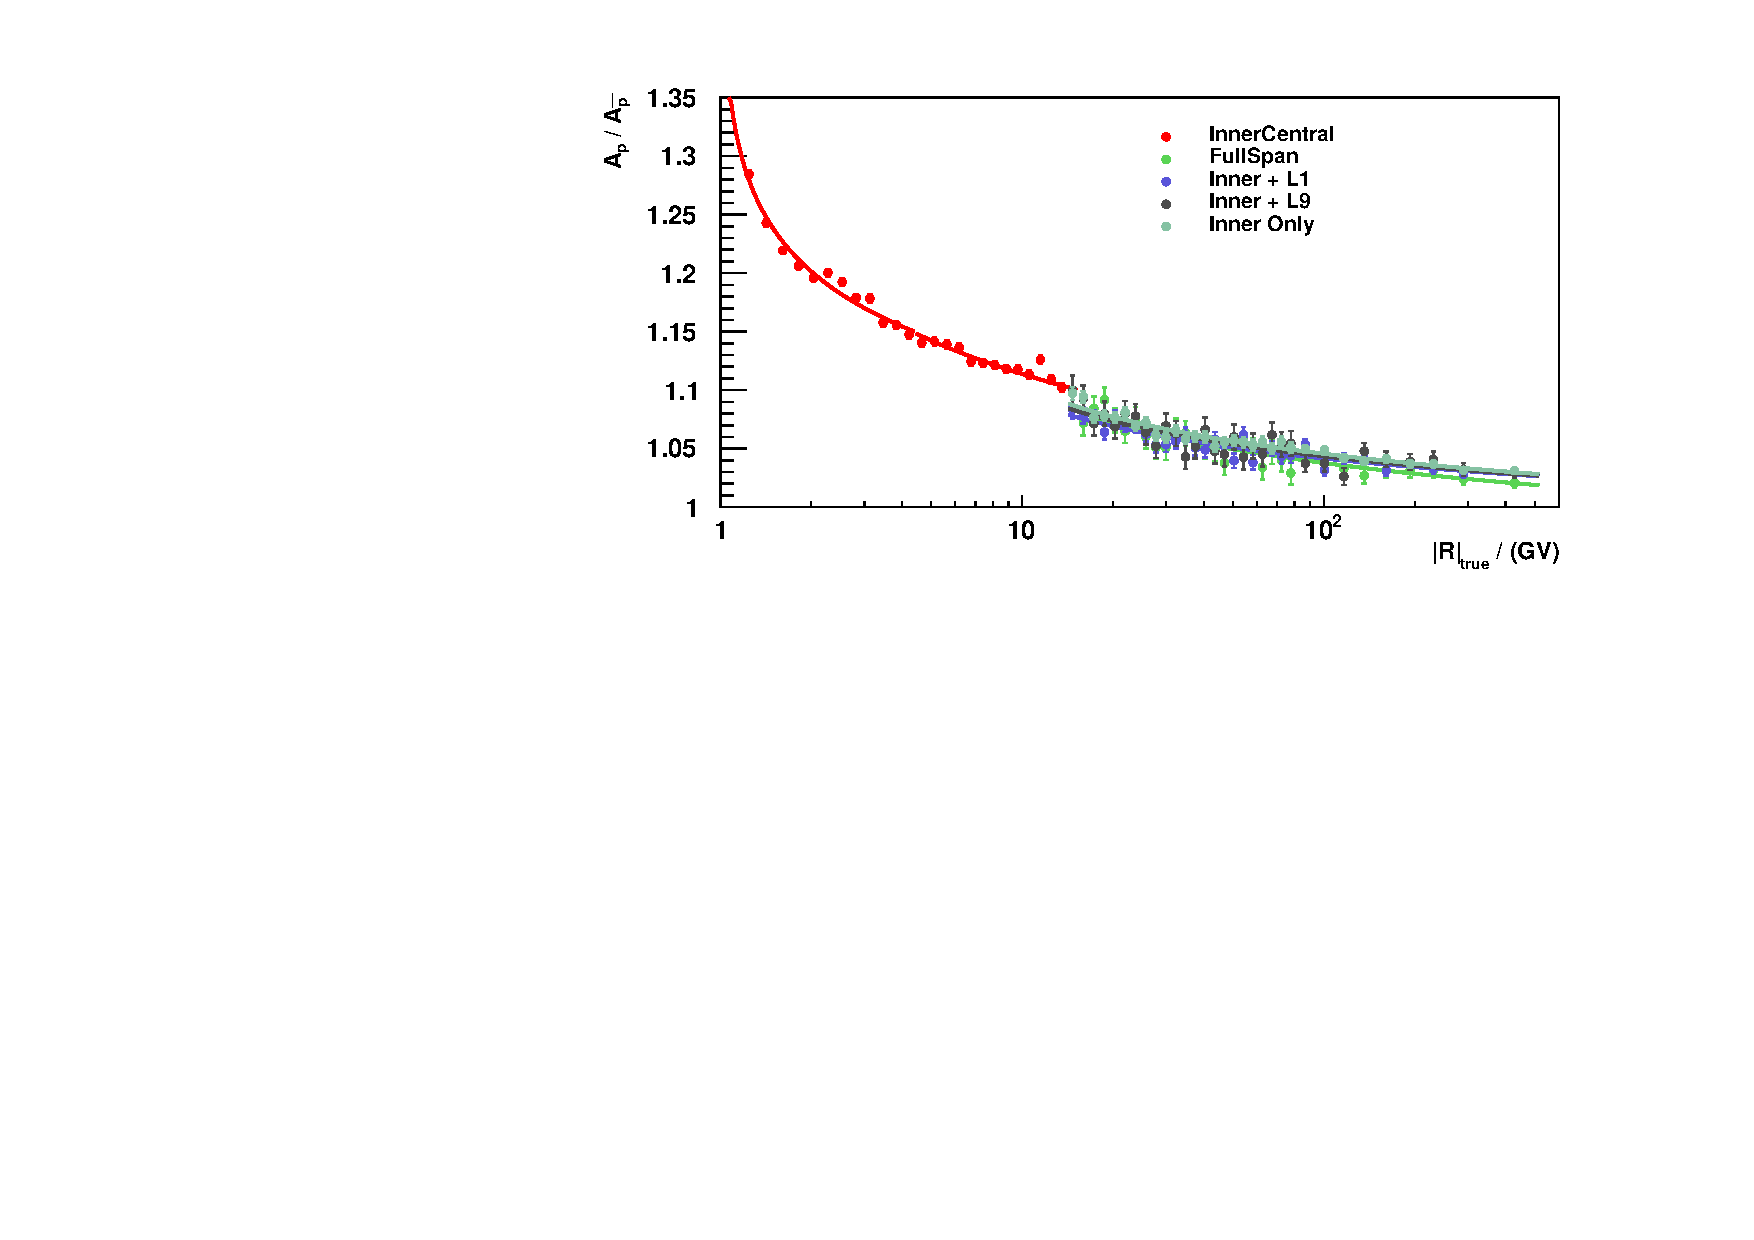
\includegraphics[width=1.00\textwidth]{Figures/chapter4/Acceptance/EffectiveAcceptanceRatio/AcceptancePlot.pdf}
\caption[Proton to antiproton effective acceptance ratios.]{Proton to antiproton effective acceptance ratios in different rigidity ranges. Due to the different selections and tracker patterns, the effective acceptance ratios are calculated individually. The uncertainty in this plot is statistical uncertainty only, the uncertainty due to the cross section will be discussed in Section \ref{SystematicUncertaintiesSection}. To have a smooth curve of the effective acceptance ratio, parameterizations are used.}
\label{TheEffectiveAcceptanceRatio}
\end{figure}

The effective acceptance ratio is rigidity-dependent and it is taken from MC first. Due to differences between ISS data and MC simulation, the effective acceptance obtained from MC needs to be corrected with the data/MC efficiency ratio. Since both of the MC determined proton effective acceptance $A^\mathrm{MC}_{p}$ and antiproton effective acceptance $A^\mathrm{MC}_{\bar{p}}$ need data/MC correction, namely $\delta_{p}$ and $\delta_{\bar{p}}$. This correction is assumed to be canceled out strictly. The same effect is valid also in the positron/electron ratio analysis \cite{ZimmermannPhDThesis}. Therefore, the effective acceptances ratio can be purely determined by MC simulations. \par

\begin{equation}
\label{EffectiveAcceptanceRatioCanceledOut}
%\frac{\Phi_{\bar{p}}}{\Phi_{p}} = \frac{N_{\bar{p}}}{N_p} \cdot \frac{A_{p}}{A_{\bar{p}}} = \frac{N_{\bar{p}}}{N_p} \cdot \frac{A^{MC}_{p}}{A^{MC}_{\bar{p}}} \cdot \frac{1+\delta_{p} }{1+ \delta_{\bar{p}} } = \frac{N_{\bar{p}}}{N_p} \cdot \frac{A^{MC}_{p}}{A^{MC}_{\bar{p}}}
\frac{A_{p}}{A_{\bar{p}}} = \frac{A^\mathrm{MC}_{p}}{A^\mathrm{MC}_{\bar{p}}} \cdot \frac{1+\delta_{p} }{1+ \delta_{\bar{p}} } = \frac{A^\mathrm{MC}_{p}}{A^\mathrm{MC}_{\bar{p}}}
\end{equation}     

Due to the different selections and different tracker patterns in three rigidity ranges, the proton to antiproton effective acceptance ratios are slightly different and determined individually. In figure \ref{TheEffectiveAcceptanceRatio}, the antiproton to proton effective acceptance ratio is shown. To avoid fluctuations in the effective acceptance ratios, the parameterizations of the effective acceptance ratios are done in different ranges individually.










\section{Measuring Time} \label{MeasuringTimeSection}

Although the measuring time is canceled in the antiproton to proton flux ratio calculation, it has to be determined due to the rigidity cutoff in the cuts and selections, which explains the low statistics in the low rigidity analysis. Also, in the time-dependent analysis, the measuring time in six Bartels Rotations helps to understand the antiproton number changes. Furthermore, in the MC simulation the rigidity cutoff is not simulated, this effect has to be corrected in unfolding. \par 

%% Definition: Measuring Time
The measuring time is the total time that all the sub-detectors are in nominal operation and could record events. Due to the detector's operation cuts and the trigger dead time, which is the time needed for readout, the measuring time is lower than the exposure time, which is the total data-taking time since the start of the experiment.   \par


%% LiveTime Fraction And Trigger 

\begin{figure}[htpb]
\centering
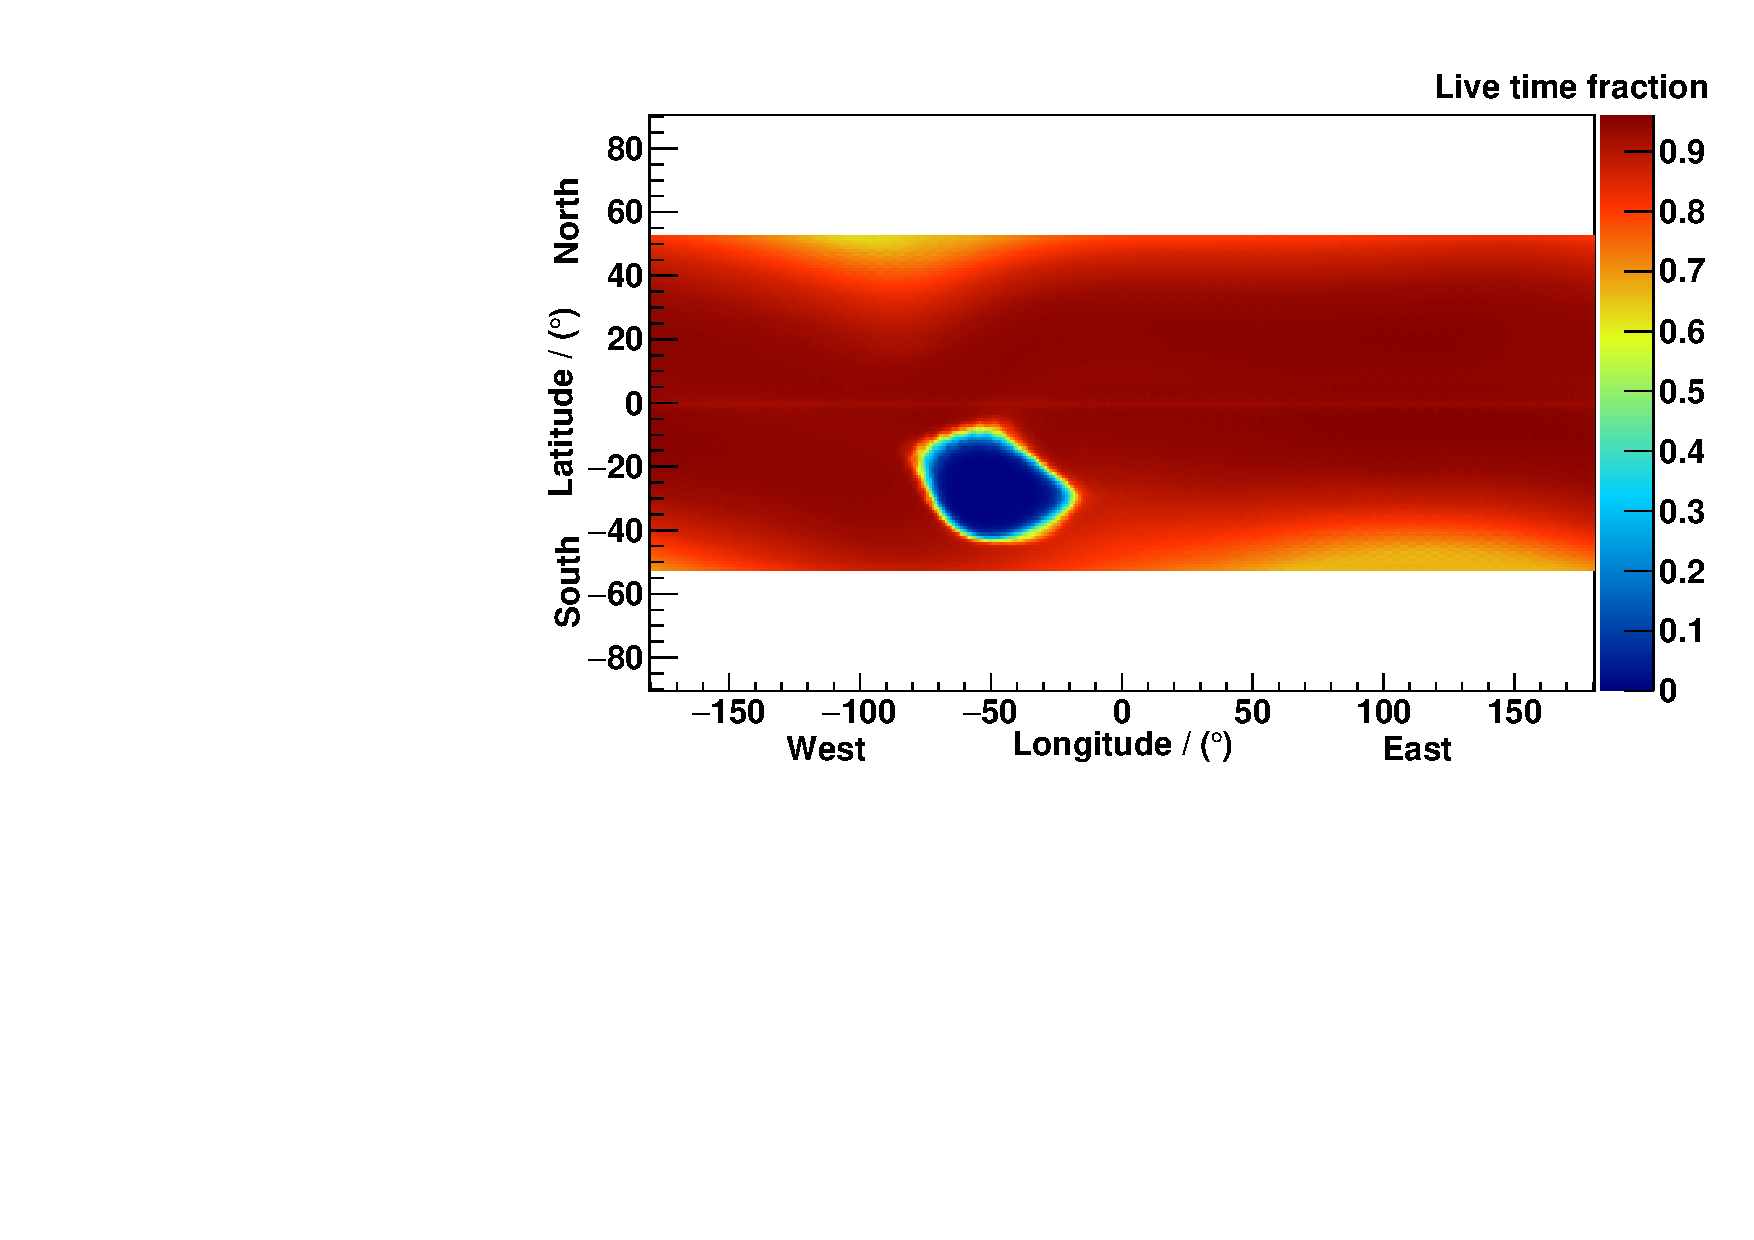
\includegraphics[width=1.0\textwidth]{Figures/chapter4/MeasuringTime/LiveTimeFractionVsISSPosition.pdf}
\caption[Live time fraction vs. ISS position.]{Live time fraction vs. ISS position. The live time fraction in the most areas is above 0.9 while in the SAA is extremely low due to plenty of low energy particles.}
\label{LiveTimeFractionVsISSPosition}
\end{figure}

Because of the trigger dead time, if the event trigger rate goes up and surpasses the threshold, then not all the events can be detected and recorded. Therefore, the live time fraction can be defined as the fraction of a second that the trigger is ready to record. Because the amount of incoming particles depends on the ISS position in the geomagnetic field, the live time fraction is close to one in most areas but less than one in high latitude areas, see figure \ref{LiveTimeFractionVsISSPosition}. Also, in the SAA, there are plenty of low energy particles going through the detector. Therefore, the trigger rate in this area is very high, and the live time fraction is very low correspondently. In figure \ref{MeasuringTimeVsLiveTime}, the measuring time as function of live time fraction is given. For the entire data-taking period, the live time fraction is mostly above 90\%.  \par
%In figure \ref{ParticlesVsTriggers}, the trigger vs. particles per trigger is presented.  \par
% In figure \ref{TriggerRateVsPosition}, the trigger rate vs ISS position is shown. 

% Start Comment out
%\begin{comment}
%\begin{figure}[]
%    \centering
%    \subfigure[]{
%        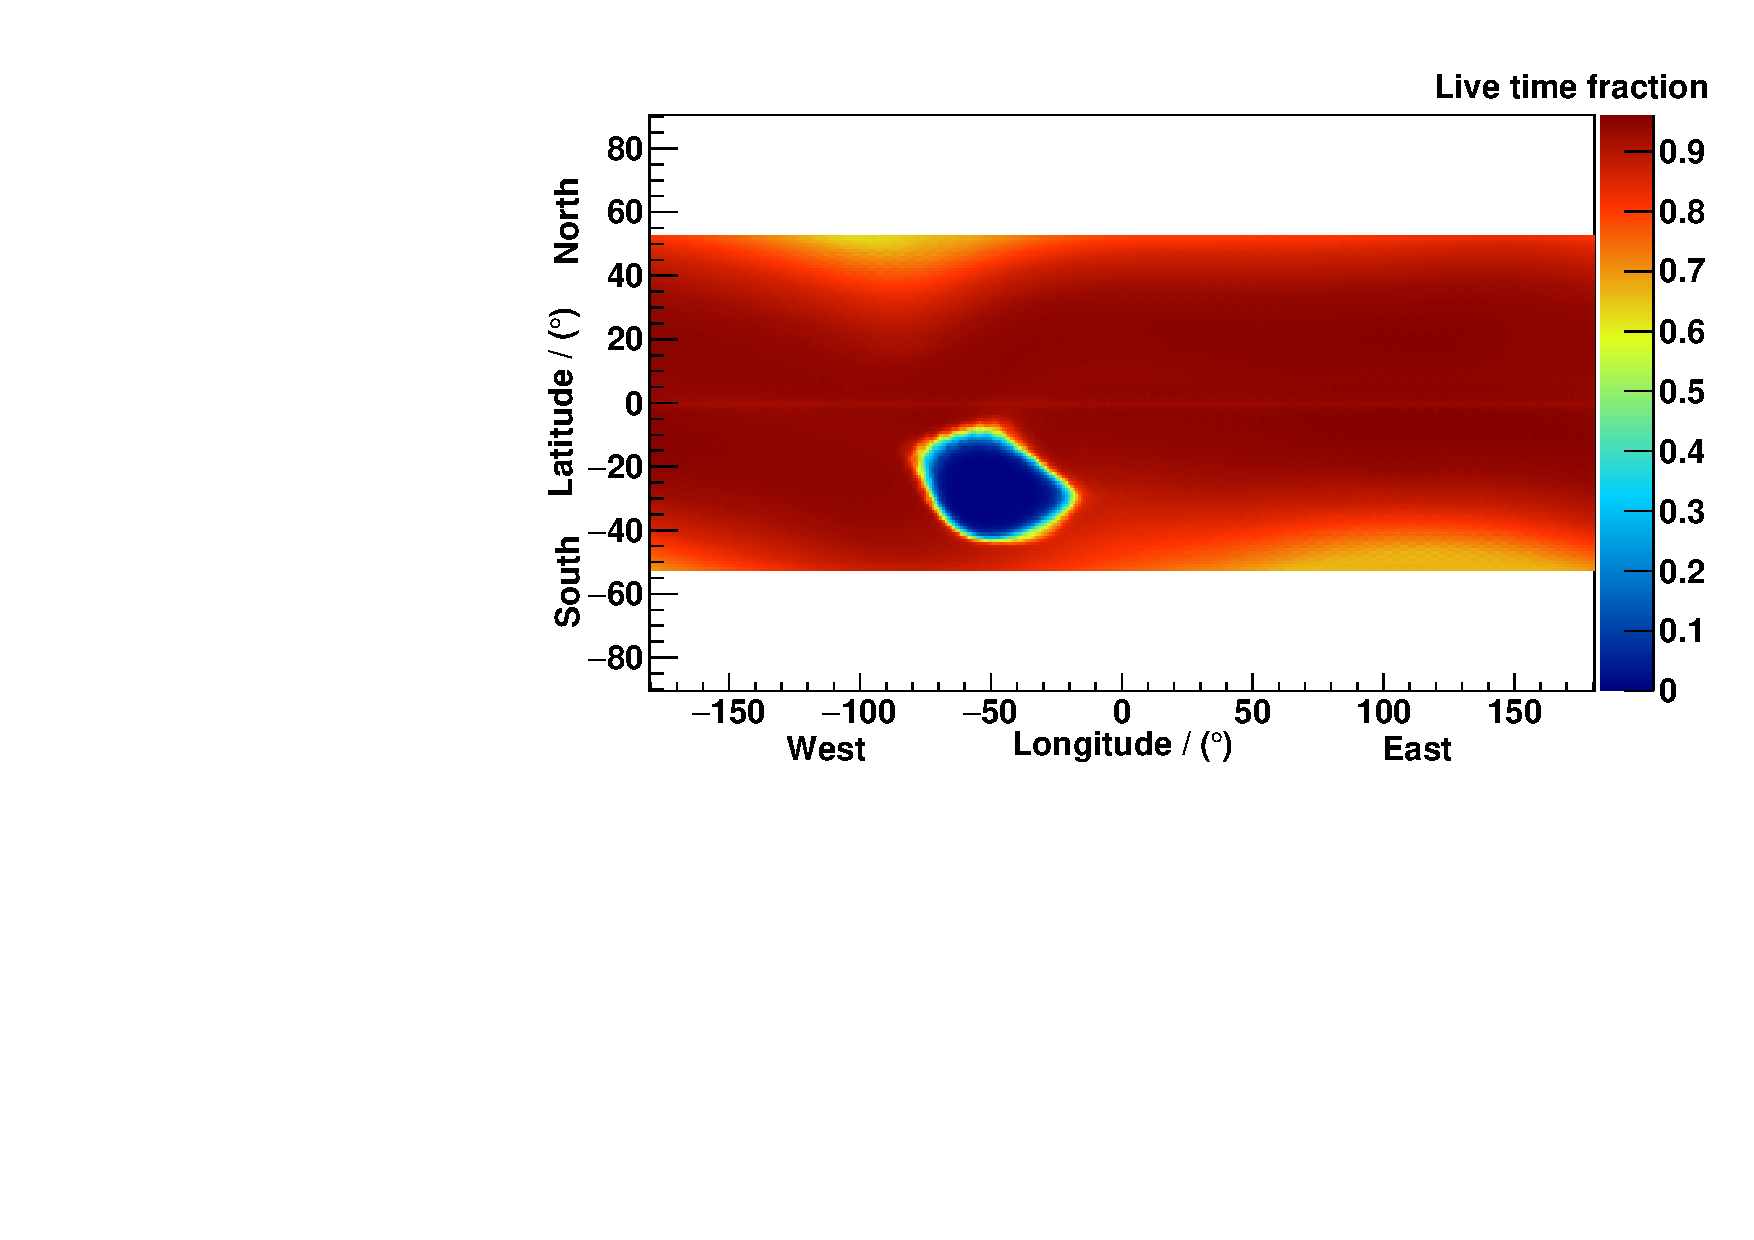
\includegraphics[width=0.47\textwidth, height=0.29\textheight]{Figures/chapter4/MeasuringTime/LiveTimeFractionVsISSPosition.pdf} 
%        \label{LiveTimeFractionVsISSPosition}
%    }
%    \subfigure[]{
%	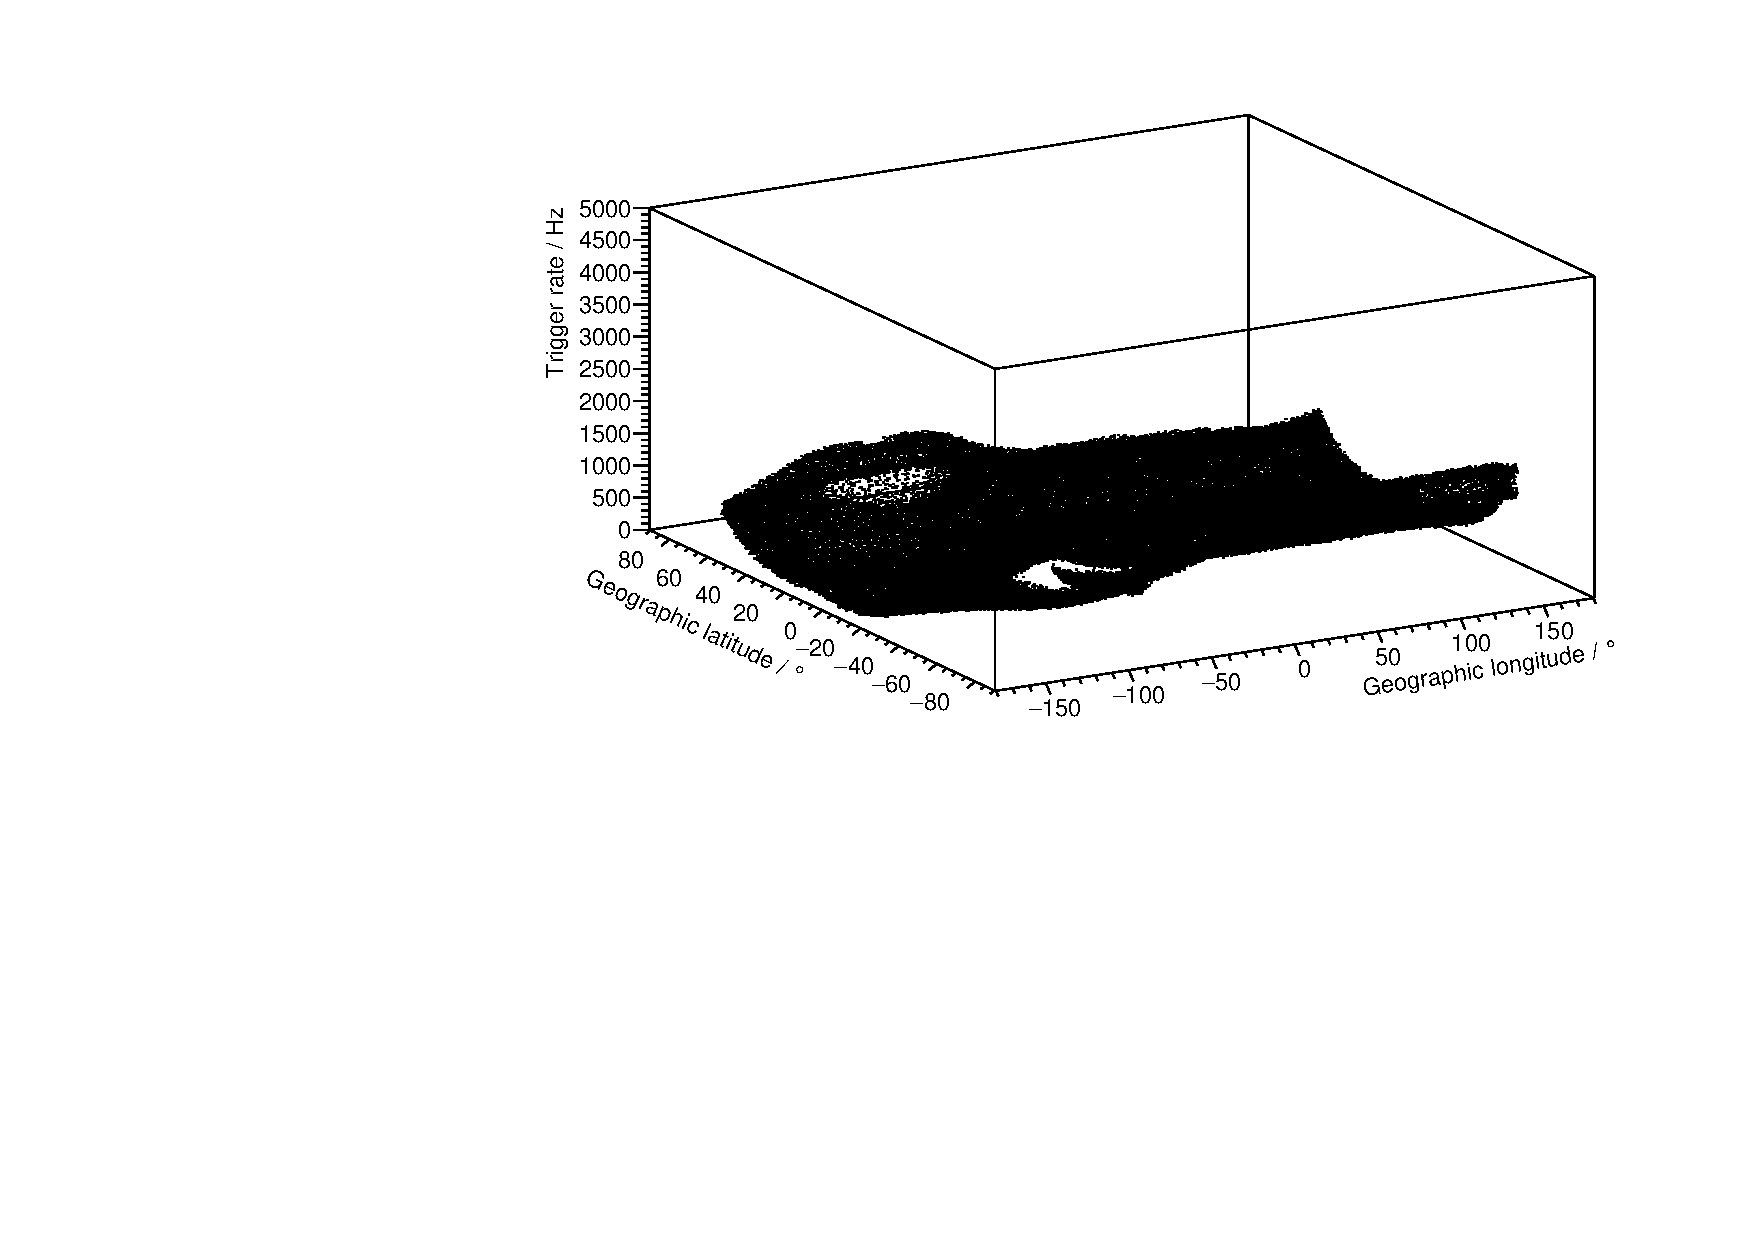
\includegraphics[width=0.47\textwidth, height=0.29\textheight]{Figures/chapter4/MeasuringTime/TriggerRateVsPosition.pdf}
%	\label{TriggerRateVsPosition}
%    }
%    \caption[]{a). Live time fraction vs. ISS position. b). Trigger rate vs. ISS position}
%\end{figure}
%\end{comment}
% End Comment out

\begin{figure}[htpb]
\centering
\includegraphics[width=1.0\textwidth]{Figures/chapter4/MeasuringTime/MeasuringTimeVsLiveTime.pdf}
\caption[Measuring time as a function of the live time fraction.]{Measuring time as a function of the live time fraction. For most of the measuring time, the live time fraction is above 0.9.}
\label{MeasuringTimeVsLiveTime}
\end{figure}
 
% Start Comment out
%\begin{comment} 
%\begin{figure}[p]
%\centering
%\includegraphics[width=1.0\textwidth, height=0.37\textheight]{Figures/chapter4/MeasuringTime/ParticlesVsTriggers.pdf}
%\caption[]{Triggers as a function of particles over trigger ratio.} 
%\label{ParticlesVsTriggers}
%\end{figure}
%\end{comment}
% End Comment out

%% Earth magnetic field 
\begin{figure}[htb]
\centering
\includegraphics[width=0.9\textwidth, height=0.37\textheight]{Figures/chapter4/MeasuringTime/Earths-Magnetic-Field-Schematic-Illustration.jpg}
\caption[Illustration of the Earth’s magnetic field.]{Illustration of the Earth’s magnetic field. The angle between the Earth’s magnetic field axis and the Earth’s rotational axis is $11.5^{\circ}$. Credit: Peter Reid, The University of Edinburgh}
\label{EarthMagneticField}
\end{figure}

Due to the Earth's magnetic field, a charged particle can be deflected before it reaches the detectors at low earth orbit, where the AMS-02 is located. The deflection power depends on the particle's rigidity and the particle's relative orientation to the magnetic field lines. \par

The Earth’s magnetic field axis is tilted at an angle of $11.5^{\circ}$ with respect to the Earth’s rotational axis, as illustrated in figure \ref{EarthMagneticField}. Therefore, the lowest rigidity threshold to penetrate the Earth's magnetic field should be a function of the Earth's location. The lowest rigidity threshold is called $\textit{rigidity cutoff}$. \par    

To get rid of these events which are deflected by the Earth's magnetic field, the following requirement is applied: 
\begin{equation}
R_\mathrm{low} > R_{c} \times f 
\end{equation}

where $f$ is the safety factor, which is set to be 1.2 in this analysis, $R_{c}$ is the cutoff rigidity,  and $R_\mathrm{low}$ is the lower edge of rigidity bin, which in the measured rigidity is classified.  \par


%% Cutoff and Measuring time
% Størmer Cutoff
For the rigidity cutoff, there are two kinds of cutoffs used in the AMS-02 collaboration: Størmer cutoff and International Geomagnetic Reference Field (IGRF) cutoff. The Størmer cutoff is only valid for the approximation of a pure dipole field. Since the geomagnetic field deviates from a pure dipole field, the IGRF cutoff takes deformations in the geomagnetic field into account and therefore more accurate. Both of the two cutoffs will be discussed in this section.\par

For the Størmer rigidity cutoff, the equation \ref{StormerCutoffCalculation} gives the formula to calculate the cutoff $R_{c}$ \cite{StormerCutOffCalculation}:  

\begin{equation}
\label{StormerCutoffCalculation}
R_{c} = \frac{M{\rm{cos}}^4\lambda}{r^2(1+\sqrt{1- \rm{sin} \epsilon \cdot \rm{sin} \delta \cdot \rm{cos}^3 \lambda } )^2}
\end{equation}

where $M$ is the geomagnetic dipole moment with a typical value of 58 \cite{StormerCutOffEquation}, $\lambda$ is the magnetic latitude, $r$ is the altitude distance from the dipole center, $\epsilon$ and $\delta$ are the zenith and azimuthal angles of the particle, respectively.

%(High: RigidityAboveIGRFCutoff(35PN|1.2).  Low:  RigidityAboveGeomagneticCutoff(25PN|1.2) )
With the cuts and selection introduced in Section \ref{DataSelectionSection}, the calculated Størmer rigidity cutoff for events with zenith angle up to 25$^{\circ}$ as a function of ISS position is given in figure \ref{StormerCutOffRigidity}. 

% Størmer Measuring Time 
The total measuring time can be obtained by integrating the live time fraction in every second of the whole data-taking period. 

\begin{figure}[hptb]
\centering
\includegraphics[width=1.0\textwidth, height=0.41\textheight]{Figures/chapter4/MeasuringTime/CutOffRigidityVsISSPosition.pdf}
\caption[The Størmer rigidity cutoff as a function of the ISS Position.]{The Størmer rigidity cutoff used in this analysis as a function of the ISS Position. The maximum value of the cutoff is less than 26 GV.}
\label{StormerCutOffRigidity}
\end{figure}


\begin{figure}[hptb]
\centering
\includegraphics[width=1.0\textwidth, height=0.41\textheight]{Figures/chapter4/MeasuringTime/Measuringtime.pdf}
\caption[The measuring time from the Størmer geomagnetic cutoff.]{The measuring time obtained from the Størmer geomagnetic cutoff. After the quality cuts and live time fraction, the resulting total measuring time is around 2488 days.}
\label{Measuringtime}
\end{figure}

\begin{figure}[htpb]
\centering
\includegraphics[width=1.0\textwidth, height=0.41\textheight]{Figures/chapter4/MeasuringTime/IGRFvsStomer.pdf}
\caption[The measuring time comparison between the Størmer and IGRF cutoffs.]{The measuring time comparison between the Størmer and IGRF cutoffs. The IGRF cutoff leads to lower measuring time.}
\label{IGRFvsStomer}
\end{figure}

After the preselection cuts introduced in Section \ref{DataSelectionSection} which ensure good operation quality of the sub-detectors, the resulting measuring time as a function of rigidity used in this analysis is shown in figure \ref{Measuringtime}. The integrated data-taking time from 20. May 2011 to 03. May 2021 is 3636 days. Due to the ISS position, detector operations like TRD gas refills and the time spent inside the SAA, the actual measuring time is around 68\% of the total data taking time. This leads to a measuring time of 2488 days above the geomagnetic cutoff.  %actual number for 2488days is: 2.1497933e+08 s

% IGRF cutoff
Another method used by the AMS-02 collaboration to calculate the rigidity cutoff is the IGRF method. To calculate the track of particle which penetrates the magnetic field, a solution is to consider the backtracing particles. With a given position and a specified rigidity, the back-trajectory of a charged particle can be traced by numerical integration through a mathematical model of the geomagnetic field, IGRF model, until the particle either reaches the interplanetary magnetic field, or intersects the atmosphere. In this way, the threshold of rigidity is the cutoff rigidity for this position.  \par
%If all the backtracing particles from a certain position and rigidity are primary particles, namely from outer space, the rigidity is the cutoff rigidity for this position. 
%The magnetic field model should be determined first in this numerical calculation of backtracing particles. One model option is the International Geomagnetic Reference Field (IGRF) model. Therefore, the name for calculating the rigidity cutoff is called IGRF method. \par
% the path of a charge particle with a specified rigidity is traced by numerical integration thrrough a mathematical model of the geomagnetic field until tthe particle either reaches the interplanetary magnetic field (allowed orbit), intersects the solid earth (forbiden orbit) or becomes 'quasi-trapped'.

% Comparison: IGRF & Stormer


Figure \ref{IGRFvsStomer} shows the comparison between the measuring time achieved from the IGRF method and the Størmer cutoff method. As shown in the figure, compared to the IGRF method, using the Størmer cutoff leads to higher statistics in the low rigidity range. This is important for the time-dependent analysis since the statistics in the fine time bin are limited. Also, using the IGRF method leads to almost zero measuring time in the first one to two rigidity bins (less than 1.16 GV). Therefore, the data could only be analyzed in the higher rigidity bins. So in this analysis, the Størmer cutoff is used to determine the measuring time though it is based on the approximation of the dipole field.

% Time-dependent Measuring Time

\begin{figure}[hptb]
\centering
\includegraphics[width=1.0\textwidth, height=0.4\textheight]{Figures/chapter4/MeasuringTime/TimeDependent/TimeDependentMeasuringTime.pdf}
\caption[The measuring time in each six Bartels Rotations time bin.]{The measuring time in each six Bartels Rotations time bin. After the middle of 2018, the measuring time in each time bin decreased due to frequent changes of the pump running status. The red line indicates the exact six Bartels Rotations (162 days).}
\label{TimeDependentMeasuringTime}
\end{figure}    

For the time-dependent analysis, the collected ISS data is divided into every six Bartels Rotations time bin. In each time bin, the total measuring time depends on the detector operation in these individual six Bartels Rotations. In figure \ref{TimeDependentMeasuringTime}, the measuring time in the 23 six Bartels Rotations time bins is shown.














%
\section{Trigger Efficiency} \label{TriggerEfficiencySection}

After the measuring time, the next ingredient needed to calculate the particle flux is the trigger efficiency. \par

%% Definition of Trigger Efficiency
The trigger efficiency is the probability for an incoming particle inside the geometric acceptance to activate the trigger system. In the AMS-02 experiment, the trigger logic is based on the response of the TOF, the ACC, and the ECAL. There are three stages in the AMS-02 trigger architecture: "Fast trigger", "Level 1 trigger" and "Level 3 trigger". The three stages are processed in sequence, namely the next stage is activated after the previous stage is fulfilled. As there is enough bandwidth to transfer the data to the ground, the "Level 3 trigger" is not activated.  \par

%% Fast trigger
There are two types of the "Fast trigger" \cite{ACCAsTrigger} stage. The first one is using the TOF. If the FTC and FTZ trigger decisions \cite{BastianPhDPaper} are fulfilled, the first type of fast trigger is set. The second one is using the ECAL. This kind of trigger is generated by showers detected by the ECAL. The first and second fast triggers are for charged particles and photons or leptons respectively. \par
%comment: the FTC:  the FTC one is generated if the CP signal (At least one TOF counter with either side having signals higher than the high threshold) is get from at least three out of the four TOF layers, the FTZ: the coincidence within 640 ns of the BZ (At least one counter with either side exceeding the super high threshold.) signals from all four layers

%% Level 1 trigger
The "Layer 1 trigger" consists of seven types of trigger conditions: \par

\begin{itemize}
\item Single charged: Has High Threshold signals (HT) in all four TOF layers, also no ACC hits. 

\item Fast ions: Has Super High Threshold (SHT) signals in all four TOF layers, also less than five ACC hits. (From 26 Feb 2016, the second condition changed to less than eight ACC hits to improve statistics.)

\item Slow ions: Has SHT signals in all four TOF layers within 640 ns. 

\item Electrons: Has HT signals in all four TOF layers, also requires at least two ECAL superlayers signals in both XZ and YZ planes. 

\item Photons: Has an ECAL shower with a zenith angle of less than $20^{\circ}$ in both XZ and YZ planes. 


\item Unbiased TOF:  Has at least three out of four TOF layer HT signals. The events triggered by this is prescaled with a factor of $f_{\mathrm{TOF}}$=100, in order to reduce the trigger rate and save bandwidth. 

\item Unbiased ECAL: Has signals in at least two ECAL superlayers in the X-Z or Y-Z plane. The events triggered by this is prescaled with a factor of $f_{\mathrm{ECAL}}$=1000, in order to reduce the trigger rate and save bandwidth. 

\end{itemize}

Among the seven types of Layer 1 triggers, the first five are called $\textit{physics triggers}$. In this analysis, only the physics triggered events are used for counting the signal numbers. To construct the flux, the last two unbiased non-physics triggers are used to calculate the trigger efficiency.

%% Calculation for double counting 
The two unbiased triggers can both fire at the same time, therefore the double-counted events should be corrected as:

\begin{equation}
\frac{1}{f_{\mathrm{TOF+ECAL}}} = \frac{1}{f_{\mathrm{TOF}}} + \frac{1}{f_{\mathrm{ECAL}}} - \frac{1} { f_{\mathrm{TOF}} \cdot f_{\mathrm{ECAL}} } 
\end{equation}

where the $f_{\mathrm{TOF}}$ and $f_{\mathrm{ECAL}}$ are the prescaling factors for unbiased TOF and unbiased ECAL triggers mentioned before, the double-counting events are prescaled with a factor of $f_{\mathrm{TOF+ECAL}} \approx 90.99$.

Once the prescaling factor is determined, the trigger efficiency $\epsilon_\mathrm{Trigger}$ can be calculated by comparing the number of physics trigger events and the unbiased non-physics trigger events:

\begin{equation}  
{\epsilon_\mathrm{Trigger}(R)}=\frac{N_\mathrm{Phys}(R)}{N_\mathrm{Phys}(R)+f_\mathrm{TOF} \cdot N_\mathrm{TOF}(R)+f_\mathrm{ECAL} \cdot N_\mathrm{ECAL}(R) + f_\mathrm{TOF+ECAL} \cdot N_\mathrm{TOF+ECAL}(R)}
\end{equation}

where $f_{\mathrm{TOF}}$, $f_{\mathrm{ECAL}}$ and $f_{\mathrm{TOF+ECAL}}$ are the prescaling factors, $N_\mathrm{Phys}$ is the number of physics trigger events, $N_\mathrm{TOF}$ and $N_\mathrm{ECAL}$ are the numbers of unbiased TOF and ECAL trigger events, $N_\mathrm{TOF+ECAL}$ is the number of events triggered by both unbiased TOF and ECAL trigger.

%% The trigger is directly taken from ISS data. \par
In figure \ref{TriggerEfficiency}, the trigger efficiency of proton is shown as an example. For the antiproton, the trigger efficiency is assumed to be the same.

\begin{figure}[H]
\centering
\includegraphics[width=1.0\textwidth, height=0.3\textheight]{Figures/chapter4/Trigger/{TriggerEff_noprescaling_B1042_antipr.pl1.1800_7.6_all_Pattern0}.pdf}
\caption{The trigger efficiency for proton events taken from MC.}
\label{TriggerEfficiency}
\end{figure}

\begin{comment}
Low and intermediate:
用的是真实的TriggerEfficiency, 该TriggerEfficiency通过“TriggerEfficiency”程序来计算得到。
    //// Load TriggerEfficiency //FIX ME: Load proton TriggerEff
    TFile *f5 = new TFile( (lowpath + string("/TriggerEff_B1042_antipr.pl1.1800_7.6_all.root")).c_str() );
    TFile *f6 = new TFile( (lowpath + string("/TriggerEff_B1042_antipr.pl1.1800_7.6_all.root")).c_str() );
    TH1F *Trig_antiproton_noprescaling_all = (TH1F*)f5->Get("TriggerEff_noprescaling");
    TH1F *Trig_proton_noprescaling_all       = (TH1F*)f6->Get("TriggerEff_noprescaling");
    TH1D *Trig_antiproton_noprescaling      = new TH1D("", "", 20, subrange_intermediate.data());
    TH1D *Trig_proton_noprescaling            = new TH1D("", "", 20, subrange_intermediate.data());
    
High:
用的是空的histogarm
实际“TriggerEfficiency”可以从Auxiliary中计算各种:通过“TriggerEfficiency”程序。
        PhysicsTriggerHisto->Write("PhysicsTriggerHisto");
        effMC_Preselection->Write("effMC_Preselection");
        effData_Preselection->Write("effData_Preselection");
        effMC_QualityCuts->Write("effMC_QualityCuts");
        effData_QualityCuts->Write("effData_QualityCuts");
        TriggerEff.Write("TriggerEff");
        TriggerEff_noprescaling.Write("TriggerEff_noprescaling");
       
\end{comment}

%% 1. Acceptance calculations do not use physics trigger cuts.  2. Trigger Efficiency canceled out.
Although the analysis is based on the physics triggered events, the cuts and selections do not include the physics trigger cut in the determination of effective acceptance in Section \ref{EffectiveAcceptanceSection}. The trigger efficiency has to be multiplied separately in the denominator of the flux. In the antiproton to proton flux ratio, the trigger efficiencies for proton $\epsilon_{p}$ and antiproton events $\epsilon_{ \overline{p} }$ cancel out in the calculation. However, the trigger efficiency is still needed in the unfolding procedure as it will be described in the next section.















\section{Unfolding} \label{unfoldingsection}

%% Reason and Definition of unfolding 
To calculate the antiproton to proton flux ratio, the number of events should be determined based on the true particle’s rigidity. However, the number of events from the template fits is determined based on the reconstructed rigidity. There are differences between these two rigidities because of the limited tracker resolution. Some events may end up in different rigidity bins, and this effect is called "bin to bin migration". To correct this effect, a procedure called $\textit{unfolding}$ is applied. Due to the different distributions of the number of events for antiproton and proton, this effect is not canceled out in the calculation of antiproton to proton flux ratio. \par

There are several methods to correct this effect and the easiest way is by matrix inversion of the migration matrix:

\begin{equation}
\label{unfoldingequation}
\hat{n} = \rm{M} \cdot n
\end{equation}

where $\hat{n}$ is the unfolded event number which is counted in the true rigidity bin, $n$ is the raw event number which is counted in the measured rigidity bin, and $\rm{M}$ is the migration matrix. The migration matrix is a 2D histogram that is obtained by filling the events in the MC simulation directly. The X axis is the reconstructed rigidity, and the Y axis is the true rigidity generated in the MC.  \par

\begin{figure}[H]
\centering
\includegraphics[width=1.0\textwidth]{Figures/chapter4/Unfolding/MM/{MM_Pattern_0}.pdf}
\caption[The migration matrix for full span at the high rigidity range for proton MC.]{The migration matrix for full span at the high rigidity range for proton MC events. The X axis is the reconstructed rigidity from the tracker and the Y axis is the true rigidity from the generated momentum in MC.}
\label{MigrationMatrix}
\end{figure}

This simple inversion method works but it is not recommended, since it gives large bin-bin correlations and magnifies statistical fluctuations. Therefore, a more complicated method called "Bayesian unfolding" is used in this work. The Bayesian unfolding method is implemented in the "RooUnfold" package in ROOT \cite{UnfoldingInRooUnfold} and is also used in the AMS-02 electron and positron analysis \cite{ZimmermannPhDThesis}. This method applies Bayes’ theorem repeatedly to invert the migration matrix and it gives more reliable results \cite{BayersUnfolding}.


%% Migration matrix
In this analysis, the signals are determined with different selections for different rigidity ranges. Also, for the different tracker patterns, the migration matrices are different due to the different tracker pattern resolutions. In figure \ref{MigrationMatrix}, the migration matrix for full span at the high rigidity range using proton simulated events is given as an example. For illustration, the histogram is normalized by ensuring the sum of probabilities in every projection along the Y axis is 1. From the figure, the diagonal elements of the matrix are the events whose true rigidity matches the reconstructed rigidity, which is the dominant part of the total events. As the rigidity increases, the bin contents of the non-diagonal elements increase too. This is due to the tracker resolution becoming worse in higher rigidity.   \par
%The migration matrix must be filled using the MC event weights to describe the migration effects of a realistic flux. 

%% MC has no rigidity cutoff. Use the shape of measuring time to correct this.
As explained in Section \ref{MeasuringTimeSection}, the collected data fulfill the rigidity cut off condition. This cutoff effect is not simulated in the MC simulation process, so it must be taken into account before we use the migration matrix. Therefore, the shape of the measuring time in figure \ref{Measuringtime} is used as a weight for the events under the rigidity cutoff.  \par

%% Underflow and overflow
%In this analysis, the template fits are performed from 0.8 GV to 525 GV. Due to the overflow and underflow of the migration matrix, the first and last bins are dropped. 


%% Compare Raw and unfolded
In this analysis, the focus is placed on the antiproton to proton ratio. Therefore, the unfolding process has to be performed for the antiproton raw event counts and the proton raw event counts respectively. The antiproton raw event counts are taken from the template fit results, and the proton raw event counts are the event counts after the cuts and selections. In figure \ref{RawUnfoldedNumbersPlot}, the raw and unfolded event counts are given for protons and antiprotons respectively.
%In figure \ref{RawUnfoldedCom}, the difference between the raw and the unfolded antiproton to proton flux ratio over the unfolded antiproton to proton flux ratio at the high rigidity range is given. The overall correction effect is less than 10\%.
%  The flux of cosmic rays is steeply falling with energy, which results in much more events at lower rigidities
% The unfolding process is performed for different tracker patterns individually.

\begin{figure}[htbp]
    \centering
    \subfigure[]{
        \includegraphics[width=1.0\textwidth, height=0.35\textheight ]{Figures/chapter4/Unfolding/RawUnfoldCompare/{NumberPlot_pass78}.pdf} 
    }
    %\hspace{-0.9cm}
    \subfigure[]{
	\includegraphics[width=1.0\textwidth, height=0.35\textheight ]{Figures/chapter4/Unfolding/RawUnfoldCompare/{ProtonNumberPlot_pass78}.pdf}
    }
    \caption[The raw and unfolded events for antiproton and proton.]{The raw and unfolded events for a) antiproton b) proton over rigidity bin width. Different migration matrices are used for different tracker patterns. Due to the different shapes of the raw event distributions for antiproton and proton, this unfolding effect can not cancel strictly.}
    \label{RawUnfoldedNumbersPlot}
\end{figure}
%The first bin is unreliable due to the underflow, therefore it is not included in the time-dependent analysis.

%\begin{figure}[H]
%\centering
%\includegraphics[width=1.0\textwidth]{Figures/chapter4/Unfolding/RawUnfoldCompare/{RawUnfoldedRatioCompare_pass7.8}.pdf}
%\caption{The difference between the raw and the unfolded antiproton to proton flux ratio over the unfolded antiproton to proton flux ratio for full span at the high rigidity range.} 
%\label{RawUnfoldedCom}
%\end{figure}










\section{Antiproton To Proton Flux Ratio} \label{SecAntiprotonToProtonRatio}

%% Time Averaged Antiproton to proton flux ratio
%In this section, the formula used for the calculation of the antiproton to proton flux ratio, which is the objective of this thesis, is given. This formula is based on equation \ref{FluxCalculationEquation} that is used for the calculation of cosmic ray fluxes, as well as the equation \ref{EffectiveAcceptanceRatioCanceledOut} that defines the ratio between the proton and antiproton effective acceptances. All the ingredients needed have been described already in the previous sections. Given the antiproton and proton flux definitions:


In this section, the antiproton to proton flux ratio is given with statistical uncertainty only. According to equation \ref{PbarOverProtonRatioEquation}, the calculated time-averaged antiproton to proton flux ratio is given with statistical uncertainty only in figure \ref{TimeAveragedRatioWithOverLapping_StaErrOnly}. Since the antiprotons are determined from different template fits in three different rigidity ranges, the results in these two overlapping ranges are also given. In the two overlapping ranges, the results are consistent with each other. In figure \ref{TimeAveragedRatioNotOverLapping_StaErrOnly}, the time-averaged antiproton to proton flux ratio without overlapping is given. The overlapping range is dealt with the best matching results. Below 4.43 GV the result in the low rigidity range is used. From 4.43 to 15.3 GV the result in the intermediate range is used. Above 15.3 GV the result in the high rigidity range is used. In figure \ref{TimeAveragedStatisticalError}, the relative statistical uncertainty of the antiproton to proton flux ratio is shown. The systematic uncertainty study will be shown in the next section. \par
 
\begin{figure}[H]
\centering
\includegraphics[width=1.00\textwidth, height=0.36\textheight]{Figures/chapter4/AntiprotonToProtonFluxRatioCalculation/TimeAveraged/{fullratio_StaErrOnly_ThisAnallysisOnly_pass78}.pdf}
\caption[The time-averaged antiproton to proton flux ratio in three rigidity ranges.]{The time-averaged antiproton to proton flux ratio in three rigidity ranges. In the two overlapping ranges, the results from different template fit methods are consistent with each other. The error bars are the statistical uncertainty only.}
\label{TimeAveragedRatioWithOverLapping_StaErrOnly}
\end{figure}

\begin{figure}[H]
\centering
\includegraphics[width=1.00\textwidth, height=0.36\textheight]{Figures/chapter4/AntiprotonToProtonFluxRatioCalculation/TimeAveraged/{fullratio_StaErrOnly_NotOverlapped_ThisAnallysisOnly_pass78}.pdf}
\caption[The time-averaged antiproton to proton flux ratio with statistical uncertainty only.]{The time-averaged antiproton to proton flux ratio with statistical uncertainty only.}
\label{TimeAveragedRatioNotOverLapping_StaErrOnly}
\end{figure}

\begin{figure}[H]
\centering
\includegraphics[width=1.00\textwidth]{Figures/chapter4/AntiprotonToProtonFluxRatioCalculation/TimeAveraged/{StaRelErr_pass78}.pdf}
\caption[The relative statistical uncertainty of the antiproton to proton flux ratio.]{The relative statistical uncertainty of the antiproton to proton flux ratio.}
\label{TimeAveragedStatisticalError}
\end{figure}


%% Time Dependent Antiproton to proton flux ratio
For the time-dependent antiproton to proton flux ratio, the calculation is based on equation \ref{TimeDependentPbarOverProtonRatioEquation}. As an example, the antiproton to proton flux ratio with statistical uncertainty only in the rigidity range of 1.92 to 2.4 GV is shown in figure \ref{TimeDependentRatio_StaErrOnly}. The corresponding statistical uncertainty is given in \ref{ExampleTimeDependenttStatisticalError}.

\begin{figure}[H]
\centering
\includegraphics[width=1.00\textwidth, height=0.4\textheight]{Figures/chapter4/AntiprotonToProtonFluxRatioCalculation/TimeDependent/{6Bartels_binmerge2_1.92_2.4_StaErrOnly}.pdf}
\caption[The antiproton to proton flux ratio in 1.92 to 2.4 GV in six Bartels Rotation.]{The antiproton to proton flux ratio in the rigidity range of 1.92 to 2.4 GV in six Bartels Rotation time bin.}
\label{TimeDependentRatio_StaErrOnly}
\end{figure}

\begin{figure}[H]
\centering
\includegraphics[width=1.00\textwidth, height=0.4\textheight]{Figures/chapter4/AntiprotonToProtonFluxRatioCalculation/TimeDependent/{StatisticalRelativeError_6Bartels_binmerge_2_1.92_2.4}.pdf}
\caption[The relative statistical uncertainty of the antiproton to proton flux ratio in 1.92 to 2.4 GV in six Bartels Rotation.]{The relative statistical uncertainty of the antiproton to proton flux ratio in the rigidity range of 1.92 to 2.4 GV in six Bartels Rotation time bin.}
\label{ExampleTimeDependenttStatisticalError}
\end{figure}









\section{Systematic Uncertainties} \label{SystematicUncertaintiesSection}

%% 4.10 The systematic uncertainty 
In this section, the systematic uncertainties are discussed. Due to the different template fit methods used in the three different rigidity ranges (low, intermediate, high), the systematic uncertainties are discussed separately for each rigidity range. \par

The antiproton to proton flux ratio is calculated according to equation \ref{PbarOverProtonRatioEquation}. There are two components in this equation: Number of events $N$ and effective acceptance $A$. These components consist the sources of the systematic uncertainties on the flux ratio. \par

\subsection{Time-averaged analysis}
%% 4.10.1. Due to Acceptance
\subsection*{Systematic uncertainty from Effective Acceptance}
The first source of systematic uncertainty is the effective acceptance. Since the effective acceptance data/MC correction cancels out, this systematic uncertainty is determined completely by the MC simulation. As the interaction cross sections of proton and antiproton are different, their effective acceptances differ too. Since the antiproton cross section measurement has much more uncertainty than proton cross section measurement, therefore is the dominant impact factor in the effective acceptance systematic uncertainty. Two dedicated antiproton MC simulation samples are generated to estimate the asymmetry of the effective acceptances. In these two antiproton MC samples, the antiproton interaction cross sections are set to nominal $\pm10\%$,  which is determined by the antiproton cross section measurements data. In figure \ref{EffectiveAcceptanceRatioWithCrossSectionVariation}, the uncertainty band shows how the effective acceptance ratio changed by varying $10\%$ of the antiproton cross section. This is the systematic uncertainty of effective acceptance. In figure \ref{SysErrFromAcceptance}, the obtained systematic uncertainty as a function of the rigidity is shown.  \par  

\begin{figure}[htpb]
\includegraphics[width=1.0\textwidth, height=0.34\textheight]{Figures/chapter4/SystematicError/Acceptance_SystemError/{EffectiveAcceptanceRatio_B1042}.pdf}
\caption[Effective acceptance ratio with antiproton cross sections varied by $\pm10\%$. ]{Proton over antiproton effective acceptance ratio with antiproton cross sections varied by $\pm10\%$. The red points are the effective acceptance ratio obtained with nominal antiproton cross section, the yellow band shows the uncertainty due to the antiproton cross section uncertainty of $10\%$.}   
\label{EffectiveAcceptanceRatioWithCrossSectionVariation}
\end{figure}

\begin{figure}[htpb]
\includegraphics[width=1.0\textwidth, height=0.34\textheight]{Figures/chapter4/SystematicError/Acceptance_SystemError/{SysRelErr_ACC_pass78}.pdf}
\caption[The systematic uncertainty from acceptance.]{The relative systematic uncertainty of the antiproton to proton flux ratio from acceptance.}
\label{SysErrFromAcceptance}
\end{figure}

%% 4.10.2. Due to event number
\subsection*{Systematic uncertainty from Event Numbers}
The second source of systematic uncertainty is the number of events. In the different rigidity ranges, the antiproton number of signal events is determined by different template fit methods given the different kinds of backgrounds relevant to each range. Therefore, the systematic uncertainty on the number of events has to be calculated separately for each rigidity range. \par

% 4.10.2.1 Low And Intermediate Range
In the low rigidity range, the antiproton signal is derived from a 2D template fit in 1/$\beta_{\rm{TOF}}$ and $\Lambda_\mathrm{TRD}$ as shown in figure \ref{LowRangeFitPlot}. A variation of the template fit range is used to estimate the template fit result. As introduced in Section \ref{TempalteFitSection}, the template fit result at 90\% signal efficiency is used in the final antiproton to proton flux ratio. To estimate the systematic uncertainty, the template fit is performed 342 times with signal efficiency from 40\% to 95\%. For the first five rigidity bins, the signal efficiency range starts from 65\% due to low statistics. Then the RMS of the results distribution is chosen as the systematic error in each rigidity bin. \par

In the intermediate rigidity range, the same logic to calculate the systematic uncertainty is used, but the difference is that the template fit in this range is a 1D template fit in $\Lambda_\mathrm{TRD}$. So in this range, the template fit is performed while varying the signal efficiency from 60\% to 100\%. \par

\begin{figure}[hptb]
    \centering
    \subfigure[]{
        \includegraphics[width=0.49\textwidth, height=0.25\textheight, trim=0cm 0cm 1.2cm 0cm, clip]{Figures/chapter4/SystematicError/FitRange_SystemError/{Ratio_vs_SignalEff_low_2.15_2.4_TimeAveraged_None_0}.pdf} 
        \label{RatoDistributions_SysErr}
    }\hspace{-10mm} 
    \subfigure[]{
	\includegraphics[width=0.49\textwidth, height=0.25\textheight, trim=0.7cm 0.6cm 0 0, clip]{Figures/chapter4/SystematicError/FitRange_SystemError/{RMS_low_2.15_2.4_TimeAveraged_None_0_LogY}.pdf}
	\label{RMS_SysErr} 
    }
    \caption[The template fit results in 2.15 to 2.4 GV while varying the signal efficiency.]{The template fit results for the antiproton to proton ratio in the rigidity bin from 2.15 to 2.4 GV while varying the signal efficiency from 40\% to 95\%. a) The template fit result distribution as a function of signal efficiency. b) The template fit result histogram. The RMS of the histogram is used as the systematic uncertainty.}      
    \label{ExampleSysErrDuetoFitRange}
\end{figure}

\begin{figure}[hptb]
\includegraphics[width=1.0\textwidth, height=0.34\textheight]{Figures/chapter4/SystematicError/FitRange_SystemError/{SysRelErr_FitRange_pass78}.pdf}
\caption[The systematic uncertainty of the antiproton to proton flux ratio from the template fit range.]{The relative systematic uncertainty of the antiproton to proton flux ratio from the template fit range.}
\label{SysErrFromTemplateFitRange}
\end{figure}

In figure \ref{ExampleSysErrDuetoFitRange}, an example of the template fit results while varying the signal efficiency is shown. The rigidity bin is from 2.15 to 2.4 GV at the low rigidity range, and the RMS of the results is used as the systematic error in this bin.

In figure \ref{SysErrFromTemplateFitRange}, the systematic uncertainty from the template fit range is shown.  \par


% 4.10.2.2 High Range
In the high rigidity range, the charge confused proton background rises dramatically with increasing rigidity. The template of the charge confused protons, which is obtained from proton MC, becomes the primary source of systematic uncertainty. \par

To estimate the systematic uncertainty due to the charge confused protons, the charge confusion level (CCLevel) between MC and ISS data is used. The CCLevel is defined as follow: 

\begin{equation}
{\rm{CCLevel}} = \frac{N_{\rm{CC Protons}}}{N_{\rm{CC Protons}}+N_{\rm{Protons}}} 
\end{equation}
where $N_{\rm{Protons}}$ is the number of charge correct protons and $N_{\rm{CC Protons}}$ is the number of charge confused protons. 

In figure \ref{CCLevelInMCandData}, the calculated CCLevels in the MC and the data are given. Similar to performed template fit, an additional cut on $\Lambda_\mathrm{CC}$ = 0.2 is applied in this plot. The CCLevel in the MC can be calculated directly by selecting the positive and negative rigidity. For CCLevel in the data, since it is impossible to extract charge confused protons from data directly, the number of charge confused protons from the template fit result is used to calculate the CCLevel.  \par

In figure \ref{chargeconfusionlevelratio}, the ISS data/MC CCLevel ratio is shown. The uncertainty band is 68\% confidence interval with a bump below 240 GV to include more points. According to the definition of the CCLevel and considering that the number of protons is much larger than the number of charge confused protons, the uncertainty in CCLevel can transfer to the uncertainty of the number of charge confused protons. For the template fit at the high rigidity range described in Section \ref{TempalteFitSection}, the number of charge confused protons can be obtained. Then the template fit is repeated again with the fixed number of charge confused protons from the first template fit result plus its uncertainty. The difference between the first template fit result and the second repeated template fit results is used as the systematic uncertainty from the charge confusion.  \par
%The uncertainty band is derived with 68\% C.L. and used as the variation of the CCLevel. 


\begin{figure}[htpb]
\includegraphics[width=1.0\textwidth, height=0.40\textheight]{Figures/chapter4/SystematicError/CC_SystemError/{CCLevel_Pattern_0_VGG16NN_CCcut_TF_0.20_525version_LogY}.pdf}
\caption[Charge confusion level in MC and data.]{Charge confusion level in MC and data. $\Lambda_\mathrm{CC}=0.2$ is applied for this plot.}
\label{CCLevelInMCandData}
\end{figure}

\begin{figure}[htpb]
\includegraphics[width=1.0\textwidth, height=0.40\textheight]{Figures/chapter4/SystematicError/CC_SystemError/{UncertaintyBand_CCLevel_Option4.3_Pattern_0_VGG16NN_CCcut_TF_0.20_525version_LinearX_ScalerBoolForPlot_True}.pdf}
%\caption[Data/MC charge confusion level ratio.]{ISS data/MC charge confusion level ratio. The yellow band indicates the 68\% confidence interval and the red dashed line is the average of the ratio points, which is very close to one.}
%\caption[Data/MC charge confusion level ratio.]{ISS data/MC charge confusion level ratio. The yellow band includes at least 67\% points and the red dashed line is the average of the ratio points, which is very close to one.}
\caption[Data/MC charge confusion level ratio.]{ISS data/MC charge confusion level ratio. The uncertainty band is 68\% confidence interval with a bump below 240 GV to include more points.}
\label{chargeconfusionlevelratio}
\end{figure}

In figure \ref{SysErrFromChargeConfusion} the systematic error due to the charge confusion is shown.

\begin{figure}[htpb]
\includegraphics[width=1.0\textwidth, height=0.34\textheight]{Figures/chapter4/SystematicError/CC_SystemError/{SysRelErr_CC_pass78_LogX}.pdf}
\caption[The relative systematic uncertainty from the charge confusion.]{The relative systematic uncertainty of the antiproton to proton flux ratio from the charge confusion.}
\label{SysErrFromChargeConfusion}
\end{figure}

% 2.3 Total systematic error
The different systematic uncertainties are added quadratically to arrive at the total systematic uncertainty. In figure \ref{SysErrTotal}, the total systematic uncertainty of the antiproton to proton flux ratio is presented.

\begin{figure}[htpb]
\includegraphics[width=1.0\textwidth, height=0.34\textheight]{Figures/chapter4/SystematicError/TotalSystemError/{SysRelErr_pass78}.pdf}
\caption[The relative total systematic error of the antiproton to proton flux ratio.]{The relative total systematic uncertainty of the antiproton to proton flux ratio.}
\label{SysErrTotal}
\end{figure}

%% Other systematic errors in PRL but not in this work.
There are some other systematic uncertainties studied in previous AMS-02 antiproton publication \cite{AMS02AntiprotonPRL2016} but not mentioned in this work, because they only contribute small uncertainties compared to the sources studied in this work. For example, the geomagnetic cutoff safe factor is set to be 1.2 in this work, and varying this value leads to a systematic uncertainty. This effect has been studied in the previous publication and contributes only 1\% at 1 GV and becomes negligible above 2 GV. Another systematic uncertainty is from the absolute rigidity scale. Due to the residual misalignment of the tracker planes, the measured rigidity could be shifted. This effect is negligible below 10 GV and gradually up to 2\% at the highest rigidity bin.

%% Total error
The statistical uncertainty is directly taken from template fit in different rigidity ranges. The total uncertainty of the antiproton to proton flux ratio is calculated by adding in quadrature the statistical and the total systematic error. \par 


%% Time-dependent Error
\subsection{Time-dependent analysis}
For the time-dependent analysis, the same procedure is followed. Since the time-dependent analysis is only performed in the rigidity range below 20 GV, the systematic uncertainties are calculated only in the low and intermediate rigidity ranges. \par

In the low and intermediate rigidity range, the systematic uncertainties are from the acceptance and fit range. Since the acceptance is taken from MC, therefore it is time-independent. The template fit is performed in each six Bartels Rotation time bin so it is time-dependent. In figure \ref{TimeDependentSystematicError}, the systematic error in the rigidity bin from 1.92 to 2.4 GV in six Bartels Rotation time bin is shown as an example. \par 

\begin{figure}[t]
\includegraphics[width=1.0\textwidth, height=0.40\textheight]{Figures/chapter4/SystematicError/TimeDependent/{RelativeBreakDownOfTotalSysError_6Bartels_binmerge_2_1.92_2.4}.pdf}
\caption[The systematic uncertainty in 1.92 to 2.4 GV in six Bartels Rotation.]{The contributions of different sources of the systematic uncertainty and the relative total systematic uncertainty of the antiproton to proton flux ratio in the rigidity bin of 1.92 to 2.4 GV in six Bartels Rotation time bin.}  
\label{TimeDependentSystematicError}
\end{figure}














